\subsection{Gradings}

These algebras inherit a grading from $\pStein_\Fp$, which is also inherited from the usual grading on weighted KLR algebras.  We will also want to consider gradings that account for wrapping around the cylinder.   The algebra $\mathring{R}$ has a grading by $\Z^I$, where a black strand with label $i$ crossing a red strand in the positive (resp. negative) direction has degree $1$ (resp. $-1$) in the $i$th component and 0 in all others.  Call this the {\bf odometer grading}.  All other crossings and dots have degree 0.  The relations (\ref{first-QH}--\ref{cost}) are obviously homogeneous for this grading.  

Consider an $\ell$-tuples of $R^{\la_i}$ modules $\mathbf{M}=(M_1,\dots, M_\ell)$.  Let $\Sigma(\mathbf{M})$ be the module spanned by diagrams where $\ell$ cyclically ordered boxes are marked with elements of the modules $M_i$, and we attach cylindrical KLR diagrams on top, subject to the relation that crossings or dots between the strands attached to a box can act on the elements of the module.

\begin{lemma}
  The module $\Sigma(\mathbf{M})$ has a basis consisting of any fixed basis of $\bigotimes M_i$, multiplied by all possible cylindrical diagrams where the strands attached to the top of a single box stay in order.
\end{lemma}
Note that in such a diagram, the leftmost strand in each group is red and thus stays in place.  Thus, all the other black strands can only sweep in the positive direction.  Also, note that strands in a group can cross, but only by ``lapping'' each other, that is, if the one on the right sweeps all the way around the back of the cylinder, it can cross over the one on the left in a rightward direction.  

If we endow with $\bigotimes M_i$ with grading 0, the module $\Sigma(\mathbf{M})$ is non-negatively graded in the odometer grading, and $\bigotimes M_i\subset \Sigma(\mathbf{M})$ is exactly the degree 0 part.
\begin{theorem}
If each $M_i$ is simple, then $\Sigma(\mathbf{M})$ has a unique graded simple quotient.  Up to grading shift, every  $\Z^I$-graded finite dimensional simple module over $\mathring{R}$ is of this form for unique $M_i$.  
\end{theorem}
\begin{proof}
If each $M_i$ is simple, then any vector of degree 0 generates $ \bigotimes M_i$ and thus all of $\Sigma(\mathbf{M})$.  Thus, a graded submodule of $\Sigma(\mathbf{M})$ is proper if and only if it is concentrated in positive degrees.  As usual, this means that the sum of two proper submodules is proper, and thus there is a unique graded simple quotient.  

If $L$ is a finite dimensional simple module, then there is a minimal degree $d$ that appears in the module.  This lowest degree part $L_d$ is a module over $R^{\la_1}\otimes \cdots \otimes R^{\la_\ell}$, since any diagram where a black strand moves across a red in the negative direction decreases degree, and thus acts trivially.  Let $\bigotimes M_i$ be any nontrivial simple submodule of $L_d$.  We thus have an induced map $\Sigma(\mathbf{M})\to L$, which is surjective, so $L$ must be the unique simple quotient of this module, and $L_d\cong \bigotimes M_i$.  This shows that $L$ is quotient of the correct form, and that $M_i$ must be unique, since it can be recovered from $L$.
\end{proof}

Thus, the gradeable simples are in bijection with $\ell$-tuples of simples $M_i$, and thus with the tensor product crystal for $\bla$.  It's not natural to thing of this as a bijection of crystals however, since the choice of a cyclic basepoint is arbitrary.  Similarly, the Grothendieck group of finite dimensional weakly gradeable (i.e. with simple constituents which are gradeable) modules is isomorphic to the tensor product of the simple representations $V(\la_i)$, but the Grothendieck group has no natural Lie algebra action.  

Note that we can apply this functor $\Sigma$ not just to $\ell$-tuples of modules over the cyclotomic quotients, but to modules over the tensor product algebras $T^{(\la_{m},\dots, \la_{m+k}}$ for lists of weights that concatenate to a rotation of the list $\bla$.  In particular, we can apply to modules over $T^\bla$ itself. 

One can easily check that this commutes with the functor of standardization: $\Sigma(\mathbb{S}^\bla(M_1,\dots, M_\ell))=\Sigma(\mathbf{M})$.  



\excise{

\subsection{The $\Z$-algebra}

Recall that $H=\End_G(V)$, and $T_H$ a maximal torus of this group.
In \cite[Def. 3.9]{WebSD}, we define for each $\nu\in X(T_HT/T)$ a
 $\mathscr{B}_{\phi+\nu}\operatorname{-}\mathscr{B}_{\phi}$
  bimodule ${}_{\phi+\nu}\mathscr{T}{}_{\phi}$ and a 
corresponding bimodule ${}_{\phi+\nu}T_{\phi}={}_{\phi+\nu}\mathscr{T}{}_{\phi}(0,0)$ over
$\mathscr{A}_{\phi+\nu}$ and $\mathscr{A}_{\phi}$.  This is a natural subquotient of the BFN algebra for $GT_H$.  This realization as a subquotient leads us to a product $ {}_{\phi+\nu}\mathscr{T}{}_{\phi+\nu'}\otimes {}_{\phi+\nu'}\mathscr{T}{}_{\phi+\nu''}\to {}_{\phi+\nu}\mathscr{T}{}_{\phi+\nu''}$.  In particular, it gives the groups ${}_mT_{n}={}_{\phi+m\nu}\mathscr{T}{}_{\phi+n\nu}$ for $m\geq n$ a $\Z$-algebra structure (in the sense of \cite{GS}).  

We can think of the projective coordinate ring of a projective variety $X$ with ample line bundle $L$ as a $\Z$-algebra with ${}_mR_n=\Gamma(X;L^{m-n})$.  Thus, a $\Z$-algebra is a non-commutative version of a projective coordinate ring.

Setting $h$ to 0 in the algebra $T$ we consider above gives a commutative $\Z$-algebra.  This defines the  projective coordinate ring of a partial resolution $\fM$ of the Coulomb branch.  This partial resolution is by construction a GIT quotient symplectic reduction of the Coulomb branch of $GT_H$ by the group  $(T_HT/T)^\vee$ with $\nu$ thought of as a character of this group.  We let $L$ be the associated ample line bundle on $\fM$.  This partial resolution was constructed in.

The $h=0$ map allows us to microlocalize the $\Z$-algebra $T$ in the sense of \cite{AVV}. The result is a sheaf of algebras $\salg_\phi$ over $\K[[h]]$ on $\fM$ quantizing the structure sheaf of this variety.  This quantization is $\bS$-equivariant, and the $\bS$-invariant sections of $\salg_\phi[h^{-1/2}]$ are isomorphic to $\EuScript{A}_\phi$.  

We can similarly define $\bS$-equivariant bimodules ${}_{\phi+m\nu}\EuScript{L}_\phi$ quantizing the line bundles associated $L^{\otimes m}$ associated to this homogeneous coordinate ring.  Given a left $\salg_\phi$-module $\mathcal{M}$, we have the $\Z$-sections \[\Gamma_\Z(\mathcal{M}):=\oplus_{m\geq 0}\Gamma(\fM;{}_{\phi+m\nu}\EuScript{L}_\phi\otimes_{\salg_\phi}\mathcal{M})\]

As in \cite[Thm 5.8]{BLPWquant}, we have a $\Z$-algebra localization theorem:
\begin{lemma}
  The category of coherent $\bS$-equivariant $\salg_\phi$-modules on $\fM$ is equivalent to the category of $\Z$-modules over ${}_{*}T_{*}$.  
\end{lemma}


\subsection{The quantum Frobenius map}

In the case where $G$ is abelian, there is a very simple Frobenius 
We can define a ``Frobenius twisted'' action of $\mathscr{A}_0$ on
polynomials via the formulas:
\begin{align}
    \vp &\mapsto \vp^p\\
    r(\acham',\acham)&\mapsto r(p\acham',p\acham)\\
    y_w&\mapsto y_w.
\end{align} 
and finally, 
\[\psi_\al\cdot f=
\begin{cases}
  0 & \al^p\nmid (f-s_{\al}f)
  \frac{f-s_{\al}f}{\al^p} & \al^p\mid (f-s_{\al}f)
\end{cases}\]
It's easy to check that these satisfy the necessary relations and that
this is compatible with the polynomial representation in the sense
that
\begin{equation}\label{eq:Fr-action}
    \Fr(a)\cdot f^p=(a\cdot f)^p.
\end{equation} 
Combined with the injectivity of the Frobenius map, this shows that
this action is faithful.  
\begin{theorem}
The variety $\fM$ is  Frobenius split. 
\end{theorem}
\begin{proof}
Consider $S_0$ with the usual Frobenius splitting $\sigma\colon S_0\to S_0$ of a polynomial ring: the unique linear map satisfying $\sigma(f^p\cdot a)=f\cdot \sigma(a)$ which is the identity in degree 0, and kills all homogeneous elements of degree not divisble by $p$.  We'll define a splitting on $\mathscr{A}_0$ by essentially running \eqref{eq:Fr-action} backwards:  we say that $\sigma(a)=b$ if we have that
\begin{equation}\label{eq:sigma-action}
    \sigma(af^p)=bf \text{ for all }f\in S_0,
\end{equation}
and $\sigma(a)=0$ if the weight of $a$ is not divisible by $p$, or if the degree of $a$ is not divisible by $p$. 

To see that this is well-defined, recall that $\C[\fM]$ has a filtration indexed by dominant coweights of $G$, with the usual dominance order, and that the $\la$ successive quotient of this filtration is a free module over $S_0^{W_\la}$, generated by a single element $\tilde{r}_{\la}$.  Furthermore, we can choose these elements so that those for non-primitive weights are just powers of the corresponding primitive vectors $\tilde{r}_{n\la}=\tilde{r}_{\la}^n$.  In this basis we obviously have $\sigma(r_{p\la}f)=r_{\la}\sigma(f)$ for $f\in S_0^{W_\la}$, and $\sigma(r_\mu)=0$ if $\mu$ is not divisible by $p$.   This shows that we have a well-defined map.

Applying this splitting to the projective coordinate ring of $\fM$ (thought of as the classical limit of $T_{*,*}$) shows that $\fM$ is Frobenius split.  
\end{proof}
By \cite[Thm. 1.1]{MR1156382}, it immediately follows that:
\begin{corollary}\label{cor:cohomology-vanishing}
We have the higher cohomology vanishing $H^i(\fM;\cO)=0$ for all $i>0$.
\end{corollary}


The polynomial ring $\Cth$ is equipped with an Artin-Schreier endomorphism $\AS\colon \Cth\to \Cth$ sending \[\vp\mapsto \vp^p-h^p\vp=\vp(\vp-h) (\vp-2h)\cdots (\vp+h).\]  Note that this endomorphism intertwines the level 1 action of $\hat {W}$ on $\ft_{\K}$ with the level 0 action, so it induces a natural map $S_0\to \Cft$.  We'll consistently use this map as our embedding of $S_0$ in $\Cft$.


Let $\mathscr{A}_1$ (resp. $\mathscr{A}_0$) denote the subcategory of $\mathscr{B}$ where we only allow the cocharacters of the form $\ft_\Z+\epsilon$ and specialize $h=1$ (resp. $h=0$).

We can easily calculate from this:
\begin{theorem}
There is a unique faithful $\Fp$-linear functor $\Fr\colon\mathscr{A}_0\to \mathscr{A}_1$ sending:
\begin{align}
    \vp &\mapsto \AS(\vp)\\
    r(\acham',\acham)&\mapsto r(p\acham',p\acham)\\
    y_w&\mapsto y_w.
\end{align} 
Thus, we have an induced map of algebras $\Fr\colon\EuScript{A}_0\to \EuScript{A}_1$.
\end{theorem}
\begin{proof}
Checking the relations is obvious.  
\end{proof}
%Note that the elements $S_0^W$ lie in the center of the categories $\mathscr{A}_0$ and $\mathscr{A}_1$, so we can base change either category by any $S_0^W$ algebra.

This is an analogue for the Coulomb branch of the  $p$-center of $U(\fg)$ for a Lie algebra in characteristic $p$.   

This Frobenius map has an analogue for $\Z$-algebras.  Let $T_0$ be the projective coordinate ring thought of as a $\Z$ algebra in the usual way: $(T_0)_{m,n}=\Gamma(\fM;L^{\otimes m-n})$.  
\begin{lemma}
  There is an inclusion $T_0\to T_1$ of $\Z$-algebras quantizing the Frobenius map on $\fM$. 
\end{lemma}
In particular, the pushforward of a $\salg_\phi$-sheaf via the
Frobenius map of varieties gives a $\bS$-equivariant coherent sheaf
over $\mathcal{O}_{\fM^{(1)}}$.  In fact, since the Frobenius map
induces an homeomorphism of topological spaces, we have an equivalence
between $\bS$-equivariant modules over $\salg_\phi$ and its
pushforward $\psalg_\phi$; of course, the latter are equivariant
coherent sheaves on $\fM^{(1)}$, and thus can be studied using the geometry of this space.}

\item the following relations around $x=1/2$ (which we draw as a
  loosely dashed
  vertical line):
\newseq
    \begin{equation*}\subeqn\label{r-dot-slide}
    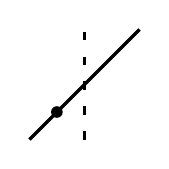
\begin{tikzpicture}[very thick,baseline,scale=.7]
  \draw(-3,0) +(-1,-1) -- +(1,1);
  \draw[loosely dashed](-3,0) +(0,-1) -- +(0,1);
\fill (-3.5,-.5) circle (3pt); \end{tikzpicture}
=
 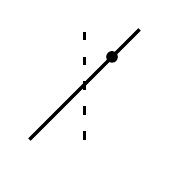
\begin{tikzpicture}[very thick,baseline,scale=.7] \draw(1,0) +(-1,-1) -- +(1,1);
  \draw[loosely dashed](1,0) +(0,-1) -- +(0,1);
\fill (1.5,.5) circle (3pt);
    \end{tikzpicture} 
\qquad \qquad     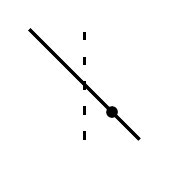
\begin{tikzpicture}[very thick,baseline,scale=.7]
  \draw(-3,0) +(1,-1) -- +(-1,1);
  \draw[loosely dashed](-3,0) +(0,-1) -- +(0,1);
\fill (-2.5,-.5) circle (3pt); \end{tikzpicture}
=
 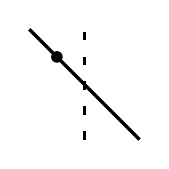
\begin{tikzpicture}[very thick,baseline,scale=.7] \draw(1,0) +(1,-1) -- +(-1,1);
  \draw[loosely dashed](1,0) +(0,-1) -- +(0,1);
\fill (.5,.5) circle (3pt);
    \end{tikzpicture} 
  \end{equation*}
 \begin{equation*}\subeqn\label{r-cost}
  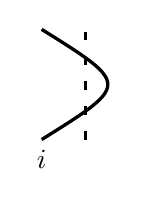
\begin{tikzpicture}[very thick,baseline,scale=.7]
    \draw (-2.8,0)  +(0,-1) .. controls (-1.2,0) ..  +(0,1) node[below,at start]{$i$};
       \draw[loosely dashed] (-2,0)  +(0,-1)--  +(0,1);
  \end{tikzpicture}
=   r_{i}\Bigg(
  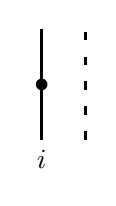
\begin{tikzpicture}[very thick,baseline,scale=.7]
 \draw[loosely dashed] (2.3,0)  +(0,-1) -- +(0,1);
       \draw (1.5,0)  +(0,-1) -- +(0,1) node[below,at start]{$i$};
       \fill (1.5,0) circle (3pt);
\end{tikzpicture}\hspace{5mm}\Bigg)\qquad \qquad
  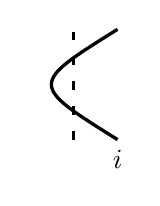
\begin{tikzpicture}[very thick,baseline,scale=.7]
          \draw[loosely dashed] (-2,0)  +(0,-1)-- +(0,1);
  \draw (-1.2,0)  +(0,-1) .. controls (-2.8,0) ..  +(0,1) node[below,at start]{$i$};\end{tikzpicture}
           =r_{i}\Bigg(\hspace{5mm}
  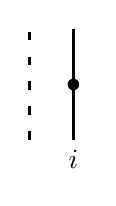
\begin{tikzpicture}[very thick,baseline,scale=.7]
    \draw (2.5,0)  +(0,-1) -- +(0,1) node[below,at start]{$i$};
       \draw[loosely dashed] (1.7,0)  +(0,-1) -- +(0,1) ;
       \fill (2.5,0) circle (3pt);\end{tikzpicture}\Bigg)
\end{equation*}
\begin{equation*}\subeqn\label{r-triple-smart}
    \begin{tikzpicture}[very thick,scale=.9,baseline]
      \draw[postaction={decorate,decoration={markings,
    mark=at position .2 with {\arrow[scale=1.3]{<}}}}] (-3,0) +(1,-1) .. controls (-4,0) .. +(-1,1) node[below,at start]{$i$}; \draw[postaction={decorate,decoration={markings,
    mark=at position .8 with {\arrow[scale=1.3]{<}}}}]
      (-3,0) +(-1,-1) .. controls (-4,0) .. +(1,1) node[below,at start]{$i$}; \draw[loosely dashed,postaction={decorate,decoration={markings,
    mark=at position .5 with {\arrow[scale=1.3]{<}}}}]
      (-3,0) +(0,-1)--  +(0,1); \node at (-1,0) {=}; \draw[postaction={decorate,decoration={markings,
    mark=at position .8 with {\arrow[scale=1.3]{<}}}}] (1,0) +(1,-1) .. controls
      (2,0) .. +(-1,1)
      node[below,at start]{$i$}; \draw[postaction={decorate,decoration={markings,
    mark=at position .2 with {\arrow[scale=1.3]{<}}}}] (1,0) +(-1,-1) .. controls
      (2,0) .. +(1,1)
      node[below,at start]{$i$}; \draw[loosely dashed,postaction={decorate,decoration={markings,
    mark=at position .5 with {\arrow[scale=1.3]{<}}}}] (1,0) +(0,-1) -- +(0,1); \node at (2.8,0)
      {$+$};        \draw (6.2,0)
      +(1,-1) -- +(1,1) node[below,at start]{$i$}; \draw (6.2,0)
      +(-1,-1) -- +(-1,1) node[below,at start]{$i$}; \draw[loosely dashed] (6.2,0)
      +(0,-1) -- +(0,1); 
\node[inner ysep=8pt,inner xsep=5pt,fill=white,draw,scale=.8] at (6.2,0){$\displaystyle \frac{r_{i}(y_k)-r_{i}(y_{k+1})}{y_k-y_{k+1}}$};
    \end{tikzpicture}
  \end{equation*}
\begin{equation*}\subeqn\label{r-triple-dumb}
    \begin{tikzpicture}[very thick,scale=.9,baseline]
      \draw[postaction={decorate,decoration={markings,
    mark=at position .2 with {\arrow[scale=1.3]{<}}}}] (-3,0) +(1,-1) .. controls (-4,0) .. +(-1,1) node[below,at start]{$j$}; \draw[postaction={decorate,decoration={markings,
    mark=at position .8 with {\arrow[scale=1.3]{<}}}}]
      (-3,0) +(-1,-1) .. controls (-4,0) .. +(1,1) node[below,at start]{$i$}; \draw[loosely dashed,postaction={decorate,decoration={markings,
    mark=at position .5 with {\arrow[scale=1.3]{<}}}}]
      (-3,0) +(0,-1)--  +(0,1); \node at (-1,0) {=}; \draw[postaction={decorate,decoration={markings,
    mark=at position .8 with {\arrow[scale=1.3]{<}}}}] (1,0) +(1,-1) .. controls
      (2,0) .. +(-1,1)
      node[below,at start]{$j$}; \draw[postaction={decorate,decoration={markings,
    mark=at position .2 with {\arrow[scale=1.3]{<}}}}] (1,0) +(-1,-1) .. controls
      (2,0) .. +(1,1)
      node[below,at start]{$i$}; \draw[loosely dashed,postaction={decorate,decoration={markings,
    mark=at position .5 with {\arrow[scale=1.3]{<}}}}] (1,0) +(0,-1) -- +(0,1); 
    \end{tikzpicture}
\qquad \text{if $i\neq j$.}
  \end{equation*}

In type $A$, we can embed these functors in a richer structure: a categorical action of $\sllhat$.    Consider the $\ell$-tuples $(s_1,\dots, s_\ell)$ with $s_k\in [0,e]$ and $\sum_{k=1}^\ell s_k=N$.  We think of these $\ell$-tuples as level $0$ weights of $\sllhat$, and thus let $\al_i=(0,\dots, 1,-1,\dots, 0)$ with $1$ in the $i$th coordinate.  
 
We associate a cylindrical KLR algebra $\mathring{R}^{\Bs}$ to each of these by taking the underlying Cartan datum of $\mathfrak{sl}_e$, and putting a red strand at $x=k/\ell$ labeled with the fundamental weight $\omega_{s_k}$.  
In \cite[Th. 4.20]{Webweb}, we constructed a categorical action of $\mathfrak{sl}_\ell$ on the corresponding linear algebras $\tilde{T}^\Bs$.  These are defined by derived tensor product with certain {\bf ladder bimodules}.  These functors commute with the left and right action by \cite[Prop. 3.8]{Webweb}.
\begin{definition}
Let $\mathsf{E}_{i},\mathsf{F}_{i}$ for $i\in \Z/\ell\Z$ be the functors $\mathring{R}^{\Bs}\to \mathring{R}^{\Bs\pm \al_i}$ obtained by reducing the categorical action of \cite[Th. 4.20]{Webweb} for $i\neq 0$, and extending using the relations 
\[\mathbb{B}_{\rho^{n}}\mathsf{E}_{i}\mathbb{B}_{\rho^{-n}}\cong \mathsf{E}_{i+n}\qquad \mathbb{B}_{\rho^{n}}\mathsf{F}_{i}\mathbb{B}_{\rho^{-n}}\cong \mathsf{F}_{i+n}.\]
\end{definition}
Just as with the braid action, we can define the corresponding bimodules directly as cylindrical KLR diagrams with certain special trivalent vertices added, by a proof identical to Proposition \ref{prop:ring-reduce}.



\begin{theorem}
 The functors $\mathsf{E}_{i},\mathsf{F}_{i}$ define a categorical action of $\sllhat$.  The action of the Rickard complexes $\Theta_i$  agree with the functors $\mathbb{B}_i$.  
\end{theorem}
\begin{proof}
First, we'll prove that we have a categorical action, assuming that $\ell>2$.  This case, every morphism and relation in the 2-category only involves two indices, and thus follows from the relations already checked in \cite[Th. 4.20]{Webweb}.  In the case of $\ell=2$, the same argument confirms that $\mathsf{E}_{i},\mathsf{F}_{i}$ define a categorical $\mathfrak{sl}_2$ action, so we only need to check that there is a natural transformation $\mathsf{E}_{1}\mathsf{E}_{0}\to \mathsf{E}_{0}\mathsf{E}_{1}$ and vice versa which define an action of the KLR algebra for $\mathfrak{\widehat{sl}}_2$.  This is easily confirmed by turning each $(s_0,s_1)$ into an $\mathfrak{\widehat{sl}}_3$ weight by adding a 0 $(s_0,s_1,0)$.  The action of $\mathsf{E}_{0},\mathsf{E}_{1},\mathsf{F}_{0}$ and $\mathsf{F}_{1}$ in $\mathfrak{\widehat{sl}}_2$ match the action of  $\mathsf{E}_{2}'\mathsf{E}_{0}',\mathsf{E}_{1}',\mathsf{F}_{0}'\mathsf{E}_{2}'$, and $\mathsf{F}_{1}'$ respectively.  The desired natural transformation $\mathsf{E}_{2}'\mathsf{E}_{0}'\mathsf{E}_{1}'\to \mathsf{E}_{1}'\mathsf{E}_{2}'\mathsf{E}_{0}'$ is the obvious pair of crossings $\psi_1\psi_2$, and similarly $\psi_1\psi_2$ in the other direction.  You can easily confirm that the $\mathfrak{\widehat{sl}}_2$-relations from the $\mathfrak{\widehat{sl}}_3$ relations, and the fact that the action of dots on either factor of $\mathsf{E}_{2}'\mathsf{E}_{0}'$ agree with the dot action on $\mathsf{E}_0$.  

Now, we wish to show the agreement of the Rickard complexes with the functors $\mathbb{B}_i$.  Again, we can assume that $\ell>2$, and reduce to the linear case.  This follows from \cite[Thm. 5.3]{Webweb}.
\end{proof}

\begin{theorem}
  The isomorphism $\widehat{\BFN}^\Bs\cong \mathring{\widehat{R}}^\Bs$
  intertwines the action of these functors with $\fE_i$ and $\fF_i$.
  In particular, the latter functors induce a categorical action of $\mathfrak{\widehat{sl}}_\ell$.
\end{theorem}
\excise{
Consider the subcategory $\stcat$ of objects in $D^b(\mathring{R}^{\Bs}\mmod)$ given by complexes where every object has a finite standard filtration which are KLR graded and odometer weakly gradeable.  These functors preserve the $\sle$ weight of modules, so the categories $\stcat\cong \oplus_\mu \stcat_\mu$ break up according to $\sle$-weight.  
\begin{theorem}
 The category $\stcat_\mu$ is closed under the action of $\sllhat$, and has Grothendieck group equal to 
 \[K^0(\stcat_\mu)\cong \bigwedge{}^{\!\!\mu_1}\C^\ell \otimes \cdots \otimes \bigwedge{}^{\!\!\mu_m}\C^\ell \]
\end{theorem}}

We can define related functors for the BFN algebra, but this requires
a bit more care.  
Choose $\ell$, an integer which satisfies $\ell \leq p$ if $\K$
has positive characteristic $p$.  Consider $\Bs\in [0,e]^\ell$.  We
associate to this tuple the BFN algebra $\BFN^{\Bs}$ where
$p_i^+(u)=\prod_{s_q=i}(u-qh-h)$ and $r_i(u)=1$.  We let $\al_i=(0,\dots,
1,-1,\dots, 0)$.  By convention, we let $\BFN^{\Bs+\frac 12
  \al_j}$  be the BFN algebra with $r_1(u) =u-jh$ and $r_i=1$ for $i>1$
$p_i^+(u)=\prod_{\lfloor s_q\rfloor =i}(u-qh-h)$.  We'll show that derived category of modules over the BFN algebras for
$\mathfrak{sl}_e$ carry a
categorical action
of $\mathfrak{sl}_\ell$ if $\K$ is characteristic 0 and
$\mathfrak{\widehat{sl}}_\ell$ if $\K$ has characteristic $p$.

We can write $\BFN^\Bs$ as the reduction of $\mathbb{\tilde T}^{\la}$
for the associated polynomial $p_i^{\pm}$, as
discussed above; we denote this algebra $\mathbb{\tilde T}^{\la;\Bs}$
to avoid confusion over which polynomial relation is used.  The algebra $\BFN^{\Bs+\frac 12
  \al_j}$ can be written as a reduction in two ways: of
$\mathbb{\tilde T}^{\la',\omega_1}$ or $\mathbb{\tilde
  T}^{\omega_1,\la'}$, but these require different polynomials on the
strand with label $\omega_1$: we must take
$u-jh$ in the first case, and $u-jh-h$ in the second.  We denote these
algebras $\mathbb{\tilde T}^{\la',\omega_1};\Bs+\frac 12
  \al_j$ or $\mathbb{\tilde
  T}^{\omega_1,\la';\Bs+\frac 12
  \al_j}$
We let $\hE_j$ denote the reduction of the web bimodule over $\mathbb{\tilde
  T}^{\omega_1,\la' ;\Bs+\frac 12
  \al_j}$ and $\mathbb{\tilde T}^{\la;\Bs}$ where we split off a
strand with label 1 to the right.  This is introduced in \cite[Def
3.7]{Webweb}.  We let $\hF_j$ be the horizontal reflection of this
bimodule, which is a bimodule over $\BFN^{\Bs-\frac
  12\al_j}\operatorname{-}\BFN^{\Bs}$.  The vertical reflection of
$\hE_j$ is a
$\BFN^{\Bs}\operatorname{-}\BFN^{\Bs+\frac 12\al_j}$-bimodule which we
denote $\Fh_j$, and the 180 degree rotation is a $\BFN^{\Bs}\operatorname{-}\BFN^{\Bs-\frac
  12\al_j}$ bimodule we denote $\Eh_j$.  For a $\BFN^{\Bs}$-module
$M$, we let
\begin{equation}
\fE_j(M)=\Eh_j\Lotimes_{\BFN^{\Bs+\frac
    12\al_j}}\hE_j\Lotimes_{\BFN^{\Bs}} M\qquad \fF_j(M)=\Fh_j\Lotimes_{\BFN^{\Bs-\frac
    12\al_j}}\hF_j\Lotimes_{\BFN^{\Bs}} M.\label{eq:EF}
\end{equation}
\begin{proposition}
  The bimodules $\hF_j, \hE_j, \Fh_j,$ and $\Eh_j$ are Harish-Chandra
  bimodules. 
\end{proposition}


If $\K$ is characteristic $p$, then we can extend to an
$\mathfrak{\widehat{sl}}_\ell$ action by defining
$\fF_0=\fF_{p}\fF_{p-1}\cdots \fF_{j+2}\fF_{j+1}$ and
$\fE_0=\fE_{j+1}\fE_{j+2}\cdots \fE_{p-1}\fE_{p}$.  In particular, if
$\ell=p$, then we can use \eqref{eq:EF} without modification.

\begin{proposition}
  The equivalence of Theorem \ref{thm:KLR-equiv} matches the functors
  $\fE_j,\fF_j$ with $\mathsf{E}_j,\mathsf{F}_j$.
\end{proposition}
\begin{proof}
  The rules for diagrams are the same as those in the isomorphism of
  Theorem \ref{thm:KLR-equiv}, and the trivalent vertex to a trivalent
  vertex in the web bimodule.
\end{proof}
\begin{proposition}\label{prop:char-0-match}
  In the characteristic 0 case, the functors $\fE_j,\fF_j$ agree with
  the categorical action of \cite{Webcatq}.  
\end{proposition}
\begin{proof}
Note that both actions are by Harish-Chandra bimodules, so it is
enough to check that they correspond to the same bimodules.  Since
Harish-Chandra modules act faithfully on category $\cO$, it's enough
to check that they act in the same way on category $\cO$.  As proven
in \cite{WebSD}, the Koszul dual of category $\cO$ for this Coulomb
branch is a tensor
  product algebra $T^\bla$ for $\mathfrak{sl}_\ell$, and by \cite{Webweb}, the action of the
  web bimodules corresponds to the usual $\mathfrak{sl}_\ell$-action
  on these categories.  Since the action of \cite{Webcatq} also
  induces this action as well by \cite{Webqui}, this shows that they match.
\end{proof}


We can use the categorical action to analyze the structure of these
categories.  The characteristic 0 case is covered in \cite{WebSD}, so
we will only consider the characteristic $p$ case.  
Let us assume for now that the weight $\mu$ given by the sum of the
labels on red and black lines is dominant.  

Now consider the case of $\Bs$ so that there are no black strands; that is, $\al_i^\vee(\mu)$ is the number of $p$ such that $s_p=i$. In this case, the algebra is one dimensional, spanned by the only possible diagram.  We let $\mathbb{V}_{\Bs}$ denote the corresponding representation.  Note that that the action of the Rickard complexes intertwine these: $\Theta_i\mathbb{V}_{\Bs}=\mathbb{V}_{s_i\cdot \Bs}.$

\begin{proposition}
 The module $\mathbb{V}_{\Bs}$ is extremal: it is killed by $\mathsf{E}_i$ if $s_i\geq s_{i+1}$ and by $\mathsf{F}_i$ if $s_{i}\leq s_{i+1}$.
\end{proposition}

Recall that by work of Kashiwara \cite{Kashlevel}, there is a
universal module with an extremal vector of this weight.  

\begin{proposition}
  The categories $D^b(\mathring{{R}}^\Bs\mmod)$ form a universal
  extremal weight categorification with respect to the action of
  $\mathsf{E}_i$ and $\mathsf{F}_i$.
\end{proposition}

% \subsection{The categorical action}
% \label{sec:categorical-action}


% Choose $\ell$, an integer which satisfies $\ell \leq p$ if $\K$
% has positive characteristic $p$.  Consider $\Bs\in [0,e]^\ell$.  We
% associate to this tuple the BFN algebra $\BFN^{\Bs}$ where
% $p_i^+(u)=\prod_{s_q=i}(u-qh-h)$ and $r_i(u)$.  We let $\al_i=(0,\dots,
% 1,-1,\dots, 0)$.  By convention, we let $\BFN^{\Bs+\frac 12
%   \al_j}$  be the BFN algebra with $r_1(u) =(u-jh)$ and $r_i=1$ for $i>1$
% $p_i^+(u)=\prod_{\lfloor s_q\rfloor =i}(u-qh-h)$. 
% The derived category of modules over the BFN algebras for
% $\mathfrak{sl}_e$ carry a
% categorical action
% of $\mathfrak{sl}_\ell$ if $\K$ is characteristic 0 and
% $\mathfrak{\widehat{sl}}_\ell$ if $\K$ has characteristic $p$.

% This action will be defined by derived tensor product with certain
% bimodules.  These are closely related to the web bimodules defined in
% \cite{Webweb}.  We define an object in the derived category of
% bimodules over $\BFN^{\Bs}$ and
% $\BFN^{\Bs+\al_i}$ given by the derived  tensor product of two halves.
% One half is given by the right module defined by BFN diagrams with a
% single vertex of the 
% Let $\hE_j$ be the  $\BFN^{\Bs+\frac 12\al_j}\operatorname{-}\BFN^{\Bs}$  bimodule of BFN diagrams where
% we add a vertex of the form 
% \begin{equation}
% \tikz[baseline,very thick,yscale=2.5,xscale=3.3]{ \draw
%   (0,-.25) -- node
%   [above, at end]{$1$} (-1,.5); \draw (0,-.25) -- node
%   [above, at end]{$j$} (-.2,.5);
% \draw
%   (0,-.25) -- node
%   [above, at end]{$2$} (-.8,.5); \draw (0,-.25) -- node
%   [above, at end]{$j-1$} (-.4,.5);
%   \draw[dashed] (0,.5) -- (0,-.5) node[above,at start]{$x=0$}; 
% %  \draw[dashed] (-2,.5) -- (-2,-.5) ; 
% \draw[loosely dashed] (0,-.25) -- (-1.2,.5) node[above,at
% end]{$x=\frac 12$};
% \node at (-.5,.4){$\cdots$};}  \label{CRR}
% \end{equation}

% As implied by the bimodule structure, we apply the relations
% (\ref{dot-slide}--\ref{r-triple-smart}) for the $p_i^\pm,r_i$
% associated to $\Bs+\frac 12\al_j$ above the triple point, and for
% $\Bs$ below it.  We let $\hF_j$ be the horizontal reflection of this
% bimodule, which is a bimodule over $\BFN^{\Bs-\frac
%   12\al_j}\operatorname{-}\BFN^{\Bs}$.  The vertical reflection of
% $\hE_j$ is a
% $\BFN^{\Bs}\operatorname{-}\BFN^{\Bs+\frac 12\al_j}$-bimodule which we
% denote $\Fh_j$, and the 180 degree rotation is a $\BFN^{\Bs}\operatorname{-}\BFN^{\Bs-\frac
%   12\al_j}$ bimodule we denote $\Eh_j$.  We for a $\BFN^{\Bs}$-module
% $M$, we let
% \begin{equation}
% \fE_j(M)=\Eh_j\Lotimes_{\BFN^{\Bs+\frac
%     12\al_j}}\hE_j\Lotimes_{\BFN^{\Bs}} M\qquad \fF_j(M)=\Fh_j\Lotimes_{\BFN^{\Bs-\frac
%     12\al_j}}\hF_j\Lotimes_{\BFN^{\Bs}} M.\label{eq:EF}
% \end{equation}


% If $\K$ is characteristic $p$, then we can extend to an
% $\mathfrak{\widehat{sl}}_\ell$ action by defining
% $\fF_0=\fF_{p}\fF_{p-1}\cdots \fF_{j+2}\fF_{j+1}$ and
% $\fE_0=\fE_{j+1}\fE_{j+2}\cdots \fE_{p-1}\fE_{p}$.  In particular, if
% $\ell=p$, then we can use \eqref{eq:EF} without modification.


This approach is particularly interesting when it is combined with the
categorical action discussed in Section \ref{sec:reduct-from-line},
and the
action of the wall-crossing functors.  Recall that the categories of
coherent sheaves on quiver varieties for a simply laced Lie algebra
carry a categorical action of the corresponding Lie algebra by
\cite{CKLquiver} and this action can extended to a copy of the
affinization of this Lie algebra by \cite{??}; note that this is a
{\it weaker} notion than a categorified loop algebra action.  We
really mean a usual categorical action for the affine root datum.
The finite $\mathfrak{sl}_\ell$ action is the classical limit of the
$\mathfrak{sl}_\ell$ action by Harish-Chandra bimodules from \cite{Webcatq} by
\cite{CDK}.  This shows that:
\begin{theorem}\label{thm:char-p-match}
  The functor $D^b(\Coh(\fM))\to D^b(\mathring{R}^{\Bs}\mmod)$
  intertwines the $\mathfrak{\widehat{sl}}_\ell$ action discussed
  above with that by the functors $\mathsf{E}_i$ and $\mathsf{F}_i$.   
\end{theorem}
\begin{proof}
  First, we check this on the finite $\mathfrak{sl}_\ell$.  In this
  case, the action on $\Coh(\fM)$ is given by taking the bimodules
  $\fE_i$ and $\fF_i$, localized to bimodules over the quantizations
  $\salg$, and taking their classical limits.  By Proposition
  \ref{prop:char-0-match}, these are the classical limits of the
  Harish-Chandra bimodules, and thus match the CKL action.  

  Furthermore, we can consider a diagram that wraps a single
  strand with positive crossings all the way around the
  cylinder in a rightward direction.  By Corollary
  \ref{cor:braidings-match}, this matches the corresponding
  wall-crossing functor, which is tensor product with the quantization
  of a line bundle $\mathcal{L}^p$. Here $\mathcal{L}$ is the line
  bundle associated to the basis cocharacter in $G_{\Bw}$ associated
  to the strand.  When we pushforward by Frobenius, we obtain the
  bimodule $\psalg\otimes \mathcal{L}$ (since the pullback of
  $\mathcal{L}$ by Frobenius is $\mathcal{L}^p$); if we use the usual
  splitting trick, the resulting bimodule over $\Hom(\cQ,\cQ)$ is
  $\Hom(\cQ,\cQ\otimes \mathcal{L})$, so transported to the category
  of coherent sheaves we simply get the functor of tensor product with
  the line bundle $\mathcal{L}$.  This confirms that we have the
  correct functors on a generating set of the category, since $\rho$
  can be obtained by starting with one of these diagrams that wraps
  one strand around the cylinder, and acting by Rickard complexes from
  the finite $\mathfrak{sl}_\ell$; once we have $\rho$, we can get
  $\mathsf{E}_0$ and $\mathsf{F}_0$.
\end{proof}
\begin{theorem}
  In the case of a type A quiver variety/S3 variety/affine
  Grassmannian slice, the action of $\pi$ on $\Coh(\fM)$ categorifies
  the monodromy of the quantum connection; that is, the
  Bezrukavnikov-Okounkov conjecture (Conjecture \ref{conj:BO}) holds. 
\end{theorem}
\begin{proof}
  First, we note that the action of the quantum connection is that
  trigonometric Casimir connection, as shown in \cite[(1.14)]{MaOk}.
  This trigonometric Casimir, acting on the $K$-theory of a quiver
  variety, is precisely the action of the quantum Weyl group in
  $\mathfrak{\widehat{sl}}_\ell$ acting via Nakajima's loop algebra
  action from \cite{Na}; since both the Casimir and quantum
  Weyl group are compatible with restrictions to Levis, we need only
  show this for $\mathfrak{sl}_2$, which is the main theorem of
  \cite{GTLsl2}\footnote{We thank Valerio Toledano-Laredo for pointing
    out this argument.}.
  
Finally, the Rickard complexes of the categorical
$\mathfrak{\widehat{sl}}_\ell$-action categorify the quantum Weyl
group action, and match the wall crossing functors by Corollary  \ref{cor:braidings-match}.


\begin{definition}
  Let $\pStein_\K'$ be the unique quotient of $\pStein_\K''$ by the
      ``codimension 1'' 
    relations
 (\ref{wall}--~\ref{demazure2}) and  the
      ``codimension 2'' 
    relations (\ref{coxeter},\ref{triple3}), given below:
\begin{align*}
    \wall(\Ba,\Bb)\wall(\Bb,\Bc)&=\hat\varphi (\Ba,\Bb,\Bc) \wall(\Ba,\Bc) \label{wall}\subeqn\\
    \mu \wall(\Ba,\Bb)& = \wall(\Ba,\Bb)\mu \label{dot-commute}\subeqn\\
    \psi_\al(\Ba)^2&=0 \label{demazure1}\subeqn\\
    \psi_\al(\Ba) (\mu)-(s_\al \mu) \psi_\al(\Ba)&=\partial_\al(\mu) \label{demazure2}.\subeqn
  \end{align*} The ``codimension 2'' 
    relations relate
the paths going around a codimension 2 intersection of hyperplanes in
the following situations:
 \begin{enumerate}[wide=0pt, widest=99,leftmargin=*, labelsep=0pt]
  \item \emph{The codimension 2 subspace is the intersection of 2 Coxeter
    hyperplanes $\cox_\al$ and $\cox_{\beta}$ which form the simple roots of a rank 2 subsystem: } 
    In this case, we have the usual
    Coxeter relations for $m=\al^\vee(\beta)\cdot \beta^\vee(\al)$:
    \begin{equation*}
      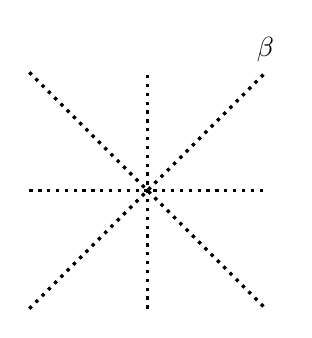
\begin{tikzpicture}[very thick,scale=1.5]
        \draw[dotted] (-1,-1) -- node[above,at
        end]{$\beta$}(1,1); \draw[dotted] (-1,1) --(1,-1);
        \draw[dotted] (-1,0) --(1,0); \draw[dotted] (0,-1) --
        node[above,at end]{$\al$} (0,1); \node at (.3,.68){${\Ba}$};
        % \draw [line width=2pt,->] (-.2,-.75) to[out=20,in=-100]
        % (.45,.6); \draw [line width=2pt,->]
        % (-.45,-.60) to[out=80,in=-160] (.2,.75);
      \end{tikzpicture}
    \end{equation*}
    \begin{equation*}
      \underbrace{\psi_\al(\Ba) \psi_\beta(\Ba)
        \psi_\al(\Ba)\cdots }_{m\text{ times}} =
      \underbrace{\psi_\beta(\Ba) \psi_\al(\Ba)
        \psi_\beta(\Ba) \cdots}_{m\text{ times}}\label{coxeter}\subeqn
    \end{equation*}
  \item \emph{The codimension 2 subspace lies in a single Coxeter
    hyperplane $\cox_\al$:}  In this case, the codimension 2
    subspace lies in some number of matter hyperplanes $H_{i_1},\dots,
    H_{i_{m-1}}$, ordered cyclically. We  label the chamber
    between $H_{i_{j-1}}$ and $H_{i_{j}}$ on the positive side of
    $\cox_\al$ by $\Ba_j$ (with the convention that
    $H_{i_0}=H_{i_m}=\cox_\al$).  Note that some of these may be
    empty.
   \begin{equation*}
      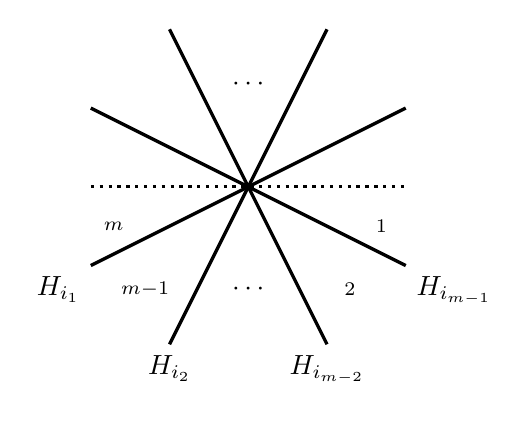
\begin{tikzpicture}[very thick]
        \draw[dotted] (-2,0) -- node [at
        start,left]{$\al$}(2,0); \draw (2,-1)-- node[below right, at
        start]{$H_{i_{m-1}}$} (-2,1); \draw (-2,-1)-- node[below left, at
        start]{$H_{i_1}$} (2,1); 
\draw (1,-2)-- node[below, at
        start]{$H_{i_{m-2}}$} (-1,2); \draw (-1,-2)-- node[below, at
        start]{$H_{i_2}$} (1,2); 
\node at (1.7,-.5)
        {${\Ba_1}$}; \node at (-1.7,-.5)
        {${\Ba_{m}}$};
\node at (1.3,-1.3)
        {${\Ba_2}$}; \node at (-1.3,-1.3)
        {${\Ba_{m-1}}$};
\node at (0,-1.3){$\cdots$}; 
\node at (0,1.3){$\cdots$};
      \end{tikzpicture}
    \end{equation*}
    
    Going from $\Ba_j$ to $s_{\al}\cdot \Ba_{m-j+1}$, there are two minimal length paths which go around the codimension 2 locus in the two opposite ways.  These don't necessarily agree, but they differ up to ``lower order terms.''
  \addtocounter{subeqn}{1}
    \begin{multline*} \subeqn \label{triple3}
      \wall(\Ba_{m-j+1},\Ba_1)\psi_\al (\Ba_1)
      \wall(\Ba_1,\Ba_j)-\wall(\Ba_{m-j+1},\Ba_m)\psi_\al
      (\Ba_m) \wall(\Ba_m,\Ba_j)\\
=\partial_{\al}(\Phi_1\cdot
      s_\al( \Phi_2)) \wall(\Ba_{m-j+1},\Ba_j)
    \end{multline*}  \addtocounter{subeqn}{-1}
    where
    \begin{align*}
\Phi_1&=\Phi( \Ba_1,\Ba_j)=\Phi(s_\al\cdot
    \Ba_{m-j+1},s_\al\cdot \Ba_{m})\\
 \Phi_2&=\Phi( \Ba_m,\Ba_{m-j+1})=\Phi(s_\al\cdot \Ba_{m},s_\al\cdot \Ba_{1}).
  \end{align*}
  \end{enumerate} Let $\widehat{\pStein}_\K'$ be the completion of
  this category with respect to the grading.  
\end{definition} 
We do not need a new relation when the codimension 2 subspace does not
lie in a root hyperplane, and thus is the intersection of some number
of matter hyperplanes, since this situation is covered by
(\ref{wall}).

As in \cite[Def. 2.12]{WebSD}, we can associate morphisms
$\tilde{\wall}_\pi\colon \Ba\to \Bb$
in $\pStein_\K'$ to a generic path $\pi\colon [0,1]\to\ft_{1,\R}$
with $\pi(0)\in \rAC_{\Ba}$ and $\pi(1)\in \rAC_{\Bb}$.   Note that
whenever this path meets a root hyperplane, by genericity, it will be
in the interior of an affine chamber $\rAC_{\Ba'}$.  Let $\al_1,\dots,
\al_m$ be the collection of root hyperplanes the path crosses, and 
$\Ba_1,\dots, \Ba_m$ be the set of chambers where it does these
crossings.  
\begin{definition}
  Let $\tilde{\wall}_\pi$ be the composition of morphisms 
\[\tilde{\wall}_\pi=\wall(\Bb,\Ba_m) \psi(\Ba_m)\wall (\Ba_{m},\Ba_{m-1})\cdots \wall(\Ba_2,\Ba_1) \psi(\Ba_1)\wall (\Ba_{1},\Ba).\]
\end{definition}

Given
$\Ba,\Bb\in \ACs$ and  $w\in \widehat{W}$, we let
$\tilde{\wall}(\Ba,\Bb,w)$ be the element given by $w^{-1}\cdot
\tilde{\wall}_\pi$ for $\pi$ a fixed generic path beginning at
$\acham_{\Ba}$ and ending at $\acham_{w\cdot \Bb}$ which crosses a
minimal number of hyperplanes.


  \begin{proposition}\label{prop:pStein-basis}
The morphism space $\Hom_{\pStein_X' }(\Ba,\Bb)$ is a free left (or
right) $S_0$ module with basis given by $\tilde{\wall}(\Ba,\Bb,w)$ as
$w$ ranges over $\widehat{W}$.  

    The kernel of the functor $\gamma'$ precisely the relations
    (\ref{wall}--\ref{triple3}).  
  The functor $\gamma'$ induces an equvialence from
  $\widehat{\pStein}_\K'$ to
  $\widehat{\mathscr{B}}_{\upsilon'}$.
  \end{proposition}

\begin{proof}
Composing the functor $\gamma'$ with the representation of Lemma
\ref{lem:frac-rep}, we have an action with formulas:
\begin{align}
\wall(\Ba,\Bb)\cdot f [t^\la]&=\varphi(\Ba,\Bb) f\cdot
                                           [t^\la]\nonumber\\
\label{eq:Y-act-frac}\psi_\al(\Ba) \cdot f [t^\la]&=\frac{s_{\al}f}{\al}[t^{s_{\al}\la}]-\frac{f}{\al}[t^{\la}]\\
w\cdot f[t^\la]&=(w\cdot f)[t^{w\la}]\nonumber\\
\mu \cdot f [t^\la]&=\mu f\cdot [t^\la]. \nonumber
  \end{align} 
This shows immediately that the elements $\tilde{\wall}(\Ba,\Bb,w)$
are linearly independent, since these act by $\tilde{\wall}(\Ba,\Bb,w)\cdot
[t^\la]=g\cdot [t^{w^{-1}\la}]+\cdots$ for $g$ a non-zero rational
function, and all other terms involving $v\cdot \la$ for $v<w^{-1}$ in
Bruhat order.  

 We can also readily calculate that the relations
 (\ref{wall}--\ref{triple3}) lie in the kernel of \eqref{eq:Y-act-frac}  as in \cite[Lemma
  2.10]{WebSD}.  This shows that they lie in the kernel of $\gamma'$ by
  the faithfulness of the action of  Lemma
\ref{lem:frac-rep}.  

To finish the proof, we need only show that in $\pStein_X'$, the elements
$\tilde{\wall}(\Ba,\Bb,w)$ span.  It's easy to see that if we consider
all generic paths $\pi$ joining the endpoints $\acham_{\Ba}$ and
$\acham_{w\cdot \Bb}$, the elements   $w^{-1}\tilde{\wall}_\pi$ span
the morphism space, since by \eqref{eq:w-commute} and
\eqref{dot-commute}, we can move elements of $\widehat{W}$ and
polynomials to the left end of any product of morphisms.

Finally, if $\pi$ is not the fixed path we used to define
$\tilde{\wall}(\Ba,\Bb,w)$, then we can isotope it to the fixed path,
remaining generic except at a finite number of points where either:
\begin{enumerate}
\item We pass through a codimension 2 intersection of hyperplanes.
\item We hit a tangency with a hyperplane, as two intersection points with
  a hyperplane cancel (note: since $\tilde{\wall}(\Ba,\Bb,w)$ is
  defined by a path with a minimal number of intersections, we can
  assume we only cancel pairs of intersections, never create them.
\end{enumerate}
The paths $\pi',\pi''$ related by (1) have that
$w^{-1}\tilde{\wall}_{\pi'}-w^{-1}\tilde{\wall}_{\pi''}$ is a sum of
similar elements for paths crossing fewer hyperplanes, by
(\ref{triple3}).  Similarly, since we are cancelling an intersection,
the relation (\ref{wall}) shows that we simply multiply by a
polynomial to account for the cancellation of the intersection points.
 Inductively, this allows us to write $w^{-1}\tilde{\wall}_\pi$ in
 terms of $\tilde{\wall}(\Ba,\Bb,w)$, using only our relations.  
\end{proof}

\excise{\begin{definition}\label{def:double-prime}
  Let $\pStein_\K''$ be the $\K$-linear category whose objects are given by $\ACs$, and whose morphisms are freely generated by symbols
  \begin{enumerate}
\item $\wall(\Ba,\Bb)\colon \Bb\to \Ba, $ for all $\Ba,\Bb\in \ACs$
\item $\mu\colon  \Ba\to \Ba$ for for all $\Ba\in \ACs$ and $\mu\in \ft^*$,
  \item $\psi_\al\colon \Ba\to \Ba$ for all $\Ba\in \ACs$ and roots
    $\al$ such that $s_\al\cdot \Ba=\Ba$
\item  a copy of $\widehat{W}_{\weights}$, which acts on objects by $w\colon
  \Ba\to w\cdot \Ba$, and commutes past the morphisms above with the
  usual relations:
  \begin{equation}
  w \wall(\Ba,\Bb) w^{-1}=\wall(w\cdot\Ba,w\cdot\Bb), \qquad\qquad
  w\psi_\al w^{-1}=\psi_{w\cdot \al}\qquad \qquad w\mu w^{-1}=w\cdot
  \mu,\label{eq:w-commute}
\end{equation}
  where in the third equation, $\widehat{W}$ acts on $\ft^*$ via the weight 0 action.
  \end{enumerate}
\end{definition}}

 \begin{itemize}
  \item we have the usual KLR relations for the polynomials:
  \newseq
%\begin{figure}[h!]


  \begin{equation*}\subeqn\label{b-black-bigon}
    \begin{tikzpicture}[very thick,scale=.9,baseline]
      \draw[postaction={decorate,decoration={markings,
    mark=at position .5 with {\arrow[scale=1.3]{<}}}}] (-2.8,0) +(0,-1) .. controls (-1.2,0) ..  +(0,1)
      node[below,at start]{$i$}; \draw[postaction={decorate,decoration={markings,
    mark=at position .5 with {\arrow[scale=1.3]{<}}}}] (-1.2,0) +(0,-1) .. controls
      (-2.8,0) ..  +(0,1) node[below,at start]{$i$}; \node at (-.5,0)
      {=}; \node at (0.4,0) {$0$};
\node at (1.5,.05) {and};
    \end{tikzpicture}
\hspace{.4cm}
    \begin{tikzpicture}[very thick,scale=.9,baseline]

      \draw[postaction={decorate,decoration={markings,
    mark=at position .5 with {\arrow[scale=1.3]{<}}}}] (-2.8,0) +(0,-1) .. controls (-1.2,0) ..  +(0,1)
      node[below,at start]{$i$}; \draw[postaction={decorate,decoration={markings,
    mark=at position .5 with {\arrow[scale=1.3]{<}}}}] (-1.2,0) +(0,-1) .. controls
      (-2.8,0) ..  +(0,1) node[below,at start]{$j$}; \node at (-.5,0)
      {=}; 
\draw (1.8,0) +(0,-1) -- +(0,1) node[below,at start]{$j$};
      \draw (1,0) +(0,-1) -- +(0,1) node[below,at start]{$i$}; 
\node[inner xsep=10pt,fill=white,draw,inner ysep=8pt] at (1.4,0) {$q_{ij}(y_1,y_2)$};
    \end{tikzpicture}
  \end{equation*}
 \begin{equation*}\subeqn\label{b-triple-dumb}
    \begin{tikzpicture}[very thick,scale=.9,baseline]
      \draw[postaction={decorate,decoration={markings,
    mark=at position .2 with {\arrow[scale=1.3]{<}}}}] (-3,0) +(1,-1) -- +(-1,1) node[below,at start]{$k$}; \draw[postaction={decorate,decoration={markings,
    mark=at position .8 with {\arrow[scale=1.3]{<}}}}]
      (-3,0) +(-1,-1) -- +(1,1) node[below,at start]{$i$}; \draw[postaction={decorate,decoration={markings,
    mark=at position .5 with {\arrow[scale=1.3]{<}}}}]
      (-3,0) +(0,-1) .. controls (-4,0) ..  +(0,1) node[below,at
      start]{$j$}; \node at (-1,0) {=}; \draw[postaction={decorate,decoration={markings,
    mark=at position .8 with {\arrow[scale=1.3]{<}}}}] (1,0) +(1,-1) -- +(-1,1)
      node[below,at start]{$k$}; \draw[postaction={decorate,decoration={markings,
    mark=at position .2 with {\arrow[scale=1.3]{<}}}}] (1,0) +(-1,-1) -- +(1,1)
      node[below,at start]{$i$}; \draw[postaction={decorate,decoration={markings,
    mark=at position .5 with {\arrow[scale=1.3]{<}}}}] (1,0) +(0,-1) .. controls
      (2,0) ..  +(0,1) node[below,at start]{$j$}; \node at (5,0)
      {unless $i=k\neq j$};
    \end{tikzpicture}
  \end{equation*}
\begin{equation*}\subeqn\label{b-triple-smart}
    \begin{tikzpicture}[very thick,scale=.9,baseline]
      \draw[postaction={decorate,decoration={markings,
    mark=at position .2 with {\arrow[scale=1.3]{<}}}}] (-3,0) +(1,-1) -- +(-1,1) node[below,at start]{$i$}; \draw[postaction={decorate,decoration={markings,
    mark=at position .8 with {\arrow[scale=1.3]{<}}}}]
      (-3,0) +(-1,-1) -- +(1,1) node[below,at start]{$i$}; \draw[postaction={decorate,decoration={markings,
    mark=at position .5 with {\arrow[scale=1.3]{<}}}}]
      (-3,0) +(0,-1) .. controls (-4,0) ..  +(0,1) node[below,at
      start]{$j$}; \node at (-1,0) {=}; \draw[postaction={decorate,decoration={markings,
    mark=at position .8 with {\arrow[scale=1.3]{<}}}}] (1,0) +(1,-1) -- +(-1,1)
      node[below,at start]{$i$}; \draw[postaction={decorate,decoration={markings,
    mark=at position .2 with {\arrow[scale=1.3]{<}}}}] (1,0) +(-1,-1) -- +(1,1)
      node[below,at start]{$i$}; \draw[postaction={decorate,decoration={markings,
    mark=at position .5 with {\arrow[scale=1.3]{<}}}}] (1,0) +(0,-1) .. controls
      (2,0) ..  +(0,1) node[below,at start]{$j$}; \node at (2.8,0)
      {$+$};        \draw (6.2,0)
      +(1,-1) -- +(1,1) node[below,at start]{$i$}; \draw (6.2,0)
      +(-1,-1) -- +(-1,1) node[below,at start]{$i$}; \draw (6.2,0)
      +(0,-1) -- +(0,1) node[below,at start]{$j$}; 
\node[inner ysep=8pt,inner xsep=5pt,fill=white,draw,scale=.8] at (6.2,0){$\displaystyle \frac{q_{ij}(y_3,y_2)-q_{ij}(y_1,y_2)}{y_3-y_1}$};
    \end{tikzpicture}
  \end{equation*}
\item the following relations around $x=0$ (which we draw as a dashed
  vertical line):
\newseq


\begin{equation*}\subeqn\label{x-triple-smart}
    \begin{tikzpicture}[very thick,scale=.9,baseline]
      \draw[postaction={decorate,decoration={markings,
    mark=at position .2 with {\arrow[scale=1.3]{<}}}}] (-3,0) +(1,-1) .. controls (-4,0) .. +(-1,1) node[below,at start]{$i$}; \draw[postaction={decorate,decoration={markings,
    mark=at position .8 with {\arrow[scale=1.3]{<}}}}]
      (-3,0) +(-1,-1) .. controls (-4,0) .. +(1,1) node[below,at start]{$i$}; \draw[dashed]
      (-3,0) +(0,-1)--  +(0,1); \node at (-1,0) {=}; \draw[postaction={decorate,decoration={markings,
    mark=at position .8 with {\arrow[scale=1.3]{<}}}}] (1,0) +(1,-1) .. controls
      (2,0) .. +(-1,1)
      node[below,at start]{$i$}; \draw[postaction={decorate,decoration={markings,
    mark=at position .2 with {\arrow[scale=1.3]{<}}}}] (1,0) +(-1,-1) .. controls
      (2,0) .. +(1,1)
      node[below,at start]{$i$}; \draw[dashed] (1,0) +(0,-1) -- +(0,1); \node at (2.8,0)
      {$+$};        \draw (6.2,0)
      +(1,-1) -- +(1,1) node[below,at start]{$i$}; \draw (6.2,0)
      +(-1,-1) -- +(-1,1) node[below,at start]{$i$}; \draw[dashed] (6.2,0)
      +(0,-1) -- +(0,1); 
\node[inner ysep=8pt,inner xsep=5pt,fill=white,draw,scale=.8] at (6.2,0){$\displaystyle \frac{p_{i,+}(y_n)-p_{i,-}(y_1)}{y_n-y_1-h}$};
    \end{tikzpicture}
  \end{equation*}
\begin{equation*}\subeqn\label{x-triple-dumb}
    \begin{tikzpicture}[very thick,scale=.9,baseline]
      \draw (-3,0) +(1,-1) .. controls (-4,0) .. +(-1,1) node[below,at start]{$j$}; \draw[postaction={decorate,decoration={markings,
    mark=at position .8 with {\arrow[scale=1.3]{<}}}}]
      (-3,0) +(-1,-1) .. controls (-4,0) .. +(1,1) node[below,at start]{$i$}; \draw[dashed]
      (-3,0) +(0,-1)--  +(0,1); \node at (-1,0) {=}; \draw[postaction={decorate,decoration={markings,
    mark=at position .8 with {\arrow[scale=1.3]{<}}}}] (1,0) +(1,-1) .. controls
      (2,0) .. +(-1,1)
      node[below,at start]{$j$}; \draw (1,0) +(-1,-1) .. controls
      (2,0) .. +(1,1)
      node[below,at start]{$i$}; \draw[dashed] (1,0) +(0,-1) -- +(0,1); 
    \end{tikzpicture}
\qquad \text{if $i\neq j$.}
  \end{equation*}
  \begin{equation*}\subeqn\label{x-triple-extra-dumb}
    \begin{tikzpicture}[very thick,scale=.9,baseline]
      \draw (-3,0) +(-1,-1) to[out=90,in=-150] node[below,at start]{$j$} +(1,1) ; \draw[postaction={decorate,decoration={markings,
    mark=at position .8 with {\arrow[scale=1.3]{<}}}}]
      (-3,0) +(-2,-1) -- +(2,1) node[below,at start]{$i$}; \draw[dashed]
      (-3,0) +(0,-1)--  +(0,1); \node at (-1,0) {=}; \draw (1,0) +(-1,-1) to [out=30,in=-90] node[below,at start]{$j$} +(1,1)
      ; \draw
      (1,0) +(-2,-1) -- +(2,1) node[below,at start]{$i$}; \draw[dashed] (1,0) +(0,-1) -- +(0,1); 
    \end{tikzpicture}
  \end{equation*}

  \end{itemize}
  
  
We wish to compare this with the extended BFN category discussed above.  For the sake of notation.  We let $z_{i,k}$ for $k=1,\dots, v_i$ denote the weights of $\C^{v_i}$ as a module over
$GL(v_i)$.  Consider the set of elements of $\ft_{\R}\subset \oplus_i \mathfrak{gl}(v_i)$ for which $z_{i,k}\not\in \Z $ and  $z_{i,k}-z_{j,m}\not\in \Z$ unless $i=j$ and $k=m$; note that this is implied by genericity for $i=j$ (due to the need to avoid translates of root hyperplanes) or when $i$ and $j$ are joined by an edge (to avoid translates of weight hyperplanes), but for simplicity, we require it for all pairs of nodes.
For each such element of $\ft_{\R}$, we define an object of the cylindrical BFN category by taking the subset of $\R/\Z$ to be the residues $z_{i,k}\pmod \Z$, each labeled with the node $i$.  Our assumptions imply that these avoid $x=0$ and each other.  

Note that this object is unchanged up to isomorphism if we deform our element in $\ft_{\R}$ without changing our desired conditions.  Furthermore, the action of the affine Weyl group leaves this subset with labeling unchanged; in fact, two elements of $\ft_{\R}$ give the same object if and only if they are conjugate under the action of the affine Weyl group.  

The claim we wish to prove is that there is an equivalence between the extended and cylindrical BFN categories; of course, the cylindrical BFN category is constructed specifically to make this theorem work.  The most important morphisms in the extended BFN category can be thought of as associated to a path from one chamber to another; we can visualize these paths as cylindrical diagrams, where the slice of the cylinder at $y=t$ is the residues mod $\Z$ of the position of the path at time $t$. 
Making this precise requires a bit more care about notation.
First, we invert the map sending an element of $\ft_{\R}$ to its residues.  For a given $\Bi$, 
we let $n_{i,k}$ be the $k$th integer in $[1,n]$ such that
$i_{n_{i,k}}=i$ (in increasing order).    We let $\tau_{i,k}$ be the dual coweight to $z_{i,k}$, thought of as an
element of the extended affine Weyl group, and let $\rho_i$ be the element of the  affine Weyl group that acts by 
\begin{equation*}
    \rho_i(z_{j,k})=\begin{cases}
    z_{j,k} & i\neq j\\
    z_{i,k-1} & i=j, k\neq 1\\
    z_{i,v_i}+1 & i=j,k=1
    \end{cases}
\end{equation*}

Given $\Bi$, consider the element $\xi_{\Bi}\in \ft\subset \oplus_i \mathfrak{gl}(v_i)$ where $z_{i,k}=n_{i,k}/n$; that is, its component in $\mathfrak{gl}(v_i)$ is the diagonal matrix $\operatorname{diag}(n_{i,1}/(n+1),\dots, n_{i,v_i}/(n+1))$.  Obviously, if we take residues in $\R/\Z$, this returns the object in the cylindrical BFN category with labels $\Bi$.

\begin{proposition}
  There is a natural functor from the cylindrical BFN category 
to the extended BFN
  $\mathscr{B}$ category with $\epsilon=0$, sending $(i_1,\dots, i_n)$ to the chamber  containing
  the point $\xi_{\Bi}$, and sending
  \begin{itemize}
  \item a dot on the $n_{i,k}$th strand to the weight $z_{i,k}$
  \item the crossing of the $p$th and $(p+1)$-st strands to
    $r(\xi_{s_p\cdot \Bi},\xi_{\Bi})$ for if $i_p\neq i_{p+1}$ and
    $p\in [1,n-1]$.
\item the crossing of the $p$th and $(p+1)$-st strands to
    $s_pu_i$ for if $i_p= i_{p+1}$ and $p\in [1,n-1]$.
\item the rightward crossing of a strand with label $i$ over $x=0$ to
  $y_{\rho_i}^{-1}r(\xi_{\rho\cdot \Bi}+\tau_{i,1},\xi_{\Bi})$, and the
  leftward to $y_{\rho_i}r(\xi_{\rho^{-1}\cdot \Bi}-\tau_{i,v_i},\xi_{\Bi})$.
  \end{itemize}
\end{proposition}



\begin{proof}
  This is clear from comparing the relations
  (\ref{b-first-QH}--\ref{x-triple-dumb}) with those of the extended
  BFN category.
  
  In particular, \begin{itemize}
      \item The relations (\ref{b-first-QH}--\ref{b-second-QH}) together with isotopy of dots past the $y$-value of crossings on differently labeled strands match precisely \cite[(3.1e)]{WebSD}.
            \item The relation (\ref{dot-slide}) follows from combining \cite[(3.1e)\& (3.2c)]{WebSD} 
      \item  The relations (\ref{b-nilHecke-1}--\ref{b-nilHecke-2}) and isotopy of dots past the $y$-value of crossings on like labeled strands matches \cite[(3.4d)]{WebSD}.

      \item The usual isotopy of diagrams follows from applications of \cite[(3.1d) \& (3.4e)]{WebSD} in cases where they are boring (there are no correction terms).  This also covers (\ref{b-triple-dumb},\ref{x-triple-dumb}--\ref{x-triple-extra-dumb}) in the cases where no two strands have the same label.
      \item The first relation of (\ref{b-black-bigon}) is \cite[(3.4a)]{WebSD}.
      \item The second relation of (\ref{b-black-bigon}) is \cite[(3.1d)]{WebSD} in the special case where we cross one of the hyperplanes for $z_{i,k}-z_{j,m}$ twice.
         \item The relation (\ref{x-cost}) is another application of \cite[(3.1d)]{WebSD}, but in the case of hyperplanes for $z_{i,k}$.  
      \item The relations (\ref{b-triple-dumb}--\ref{b-triple-smart}, \ref{x-triple-smart}--\ref{x-triple-extra-dumb}) match \cite[(3.4e)]{WebSD} for the two different types of weight hyperplanes.
  \end{itemize}
  This confirms the full list of relations and thus proves the theorem.
\end{proof}

\begin{equation*} 
       \tikz[very thick,scale=.8,baseline]{
\draw (1.2,2.5)-- (1.2,-2.5) node[at start,above,scale=.8]{$z_1=\frac{1}{2}$}; \draw (-1.2,2.5)--
(-1.2,-2.5) node[at start,above,scale=.8]{$z_1=-\frac{1}{2}$};
\draw (2.5,1.2)-- (-2.5,1.2) node[at start,right,scale=.8]{$z_2=\frac{1}{2}$}; \draw (2.5,-1.2)--
(-2.5,-1.2) node[at start,right,scale=.8]{$z_2=-\frac{1}{2}$}; 
 \draw[dotted] (-2.5,-2.5) -- node[above right,at
        end,scale=.8]{$\alpha=0$}(2.5,2.5); 
 \draw[dotted] (-2.5,-.1) -- node[left ,at
        start,scale=.8]{$\alpha=-1$}(.1,2.5); 
 \draw[dotted] (-.1,-2.5) -- node[right,at
        end,scale=.8]{$\alpha=1$}(2.5,.1); 
\draw[->,dashed] (-.4,.4) to (-2,-.4);
}\qquad \leftrightarrow \qquad
       \tikz[very thick,xscale=1.5,baseline]{
          \draw[fringe] (-1,-1)-- (-1,1);
          \draw[fringe] (1,1)-- (1,-1);
           \draw (.4 ,1) to (1,0);
           \draw (-1,0) to(-.4,-1);
        \draw (-.4 ,1) to (.4,-1);

        }
\end{equation*}

We have a category $\widehat{\BFN}$ whose objects are sequences $\Bi$
and weights $(a_1,\cdots,a_n)$ that give generalized eigenvalues of
the dots in $\K$, with morphisms $(\Bi,\Ba)\to (\Bj,\Bb)$  given by
the coarsest completion of $e(\Bi)\BFN e(\Bj)$ where $y_k$ acts on the
left with generalized eigenvalue $a_k$ and on the right with
generalized eigenvalue $b_k$.  As in \cite{WebSD}, finite dimensional representations of
the category $\widehat{\BFN}$ are equivalent to weight representations of $\BFN$.

Pick an order on $\Gamma$, and number the vertices $1,\dots, r$; for
simplicity, we orient the edges in the increasing direction. Let $\Bi$
be the sequence where the labels are in increasing order.  Let $e_0$
be the idempotent endomorphism of this sequence where we multiply each
group of strands with the same label with a primitive idempotent in
the nilHecke algebra.
If we take $b_e=-\nicefrac{a_{ij}}{2}-p$ for $p=1,\dots, -a_{ij}$ for
the $a_{ij}$ edges joining $i$ and $j$, then \cite[Thm. B.18]{BFNplus} shows that:
\begin{proposition}
The endomorphisms of $e_0$ are isomorphic to the truncated shifted
Yangian for $\Gamma$.  
\end{proposition}
Thus, this category is another framework in which to view the Yangian,
and there is a natural quotient functor from weight modules over
$\BFN$ to those of the Yangian, given by multiplication by $e_0$.    We'll develop this further in \cite{KTWWY2} to better understand the representation theory of Yangians. 


 \begin{definition}\label{def:cyl-Stendhal}
  A {\bf cylindrical Stendhal diagram} is a collection of finitely many
  oriented curves in $\R/\Z\times [0,1]$ (which are all colored
  black). Each curve is labeled with $i\in \Gamma$ and decorated with
  finitely many dots.  The diagram must be locally of the
  form 
with each curve oriented in the negative direction.  The curves must
meet the circles at
$y=0$ and $y=1$ at distinct points with $x\neq 0$. We consider these
up to isotopy preserving the conditions above.  
\end{definition}

As before, we'll draw these on the page in the rectangle $[0,1]\times [0,1]$ with seams on the left and right side of the diagram where we should glue to obtain the cylindrical diagram.  An example of such a diagram is \begin{equation*} 
       \tikz[very thick,xscale=1.5]{
          \draw[fringe] (-1,-1)-- (-1,1);
          \draw[fringe] (1,1)-- (1,-1);
          \draw[wei] (-.8,-1)--node[below, at start ]{$\la$} (-.8,1);
          \draw[wei] (.4 ,-1)--node[below, at start ]{$\mu$} (.4,1);
\draw (-1,.2) to[out=30,in=-90] node[above, at end]{$i$} (.2,1);
           \draw (.6 ,-1) to[out=90,in=-150] node[below, at start ]{$i$}(1,.2);
           \draw (-1,-.2) to[out=-30,in=90]node[below, at end ]{$k$} (-.5,-1);
           \draw (-.2 ,1) to[out=-90,in=150] node[midway,circle,fill=black,inner sep=2pt]{} node[above, at start ]{$k$}(1,-.2);
           \draw (-.2,-1) to[out=90,in=-90] node[below, at start ]{$i$} node[above, at end]{$i$} (-.5,1);
        }
\end{equation*}

We fix the number of black strands to be $n$.  Fix one of our red strands to be ``first'' as a reference point, and number the others in terms of increasing $x$-value. We will similarly number the black strands starting at this red strand, and as in the linear case, let $y_k$ denote a dot on the $k$th black strand, $\psi_k$ a crossing of the $k$th and $k+1$st black strands.  As in the linear case, we let $i_k$ be the label on the $k$th black strand, and let  $\kappa(j)$ denote the integer such that the $j$th red strand is between the $\kappa(j)$th and $(\kappa(j)+1)$st black strands.  Note that we have chosen our numbering so that $\kappa(1)=0$. 

Consider an infinite direct sum of polynomial rings in the variables $Y_i$, one for each choice of $\Bi, \kappa$ and an $n$-tuple of integers $(g_1,\dots, g_n)$.  The latter serve as ``odometers'' to track how strands wrap around the cylinder.  As usual, this action is defined by:
  \begin{equation*}
\begin{tikzpicture}[scale=.4,baseline]
\draw[wei] (-1,-1) -- (1,1) node[at start,below]{
$\la$} node[at end,above]{
$\la$};
\draw[very thick] (1,-1) -- (-1,1) node[at start,below]{
$i$} node[at end,above]{
$i$};
%\draw[very thick,|->] (1.5,0) -- (2.5,0);
\node at (2.7,0) {$\bullet\: f= f$ } ;
\end{tikzpicture}\qquad \qquad
\begin{tikzpicture}[scale=.4,baseline]
\draw[wei] (1,-1) -- (-1,1) node[at start,below]{
$\la$} node[at end,above]{
$\la$};
\draw[very thick] (-1,-1) -- (1,1) node[at start,below]{
$i$} node[at end,above]{
$i$};
\node at (3.7,0) {$\bullet\: f=Y_k^{\la^i}\cdot f$ } ;
\end{tikzpicture}\qquad \qquad
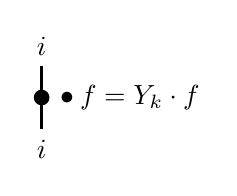
\begin{tikzpicture}[scale=.4,baseline]
\draw[very thick] (1,-1) -- (1,1) node[at start,below]{
$i$} node[at end,above]{
$i$} node[circle,midway,fill,inner sep=2pt]{};
\node at (3.8,0) {$\bullet\: f= Y_k\cdot f$ } ;
\end{tikzpicture}
  \end{equation*}
\begin{equation*}
  \begin{tikzpicture}[scale=.4]
\draw[very thick] (1,-1) -- (-1,1) node[at start,below]{
$j$} node[at end,above]{
$j$};
\draw[very thick] (-1,-1) -- (1,1) node[at start,below]{
$i$} node[at end,above]{
$i$};
\node at (7.5,0) {$\bullet\: f=\begin{cases}
 P_{ji}(Y_k,Y_{k+1}) f^{s_k} & i\neq j\\
 \displaystyle \frac{f^{s^k}- f}{Y_{k+1}-Y_{k}} & i=j  
\end{cases}$ } ;
\end{tikzpicture}
\end{equation*}
The only subtlety is that when a black strand crosses leftward over the first red strand, it goes from first to last and we must cyclically permute the variables $Y_*$ and labels $i_*$ as well as the odometer with a shift; it becomes $(g_2,\dots, g_n,g_1-1)$.  Crossing the other direction reverses this process, as well as multiplying by the required power of $Y_1$.  

The use of the ``odometer'' is a bit annoying, but necessary, since otherwise, this action would not be faithful. For example, the diagram that wraps all strands one step around the cylinder would simply match multiplication by a polynomial; in our representation, these act differently, since the former diagram increases the odometer of each strand, while the latter leaves it unchanged.   

\excise{ Consider an infinite family of variables $Y_i$ for $i\in \Z$.  We will define a representation of our category that sends each idempotent to a ring $S$ defined to be finite formal sums of formal (possibly infinite) products of polynomials such that for any finite set of variables, only finitely many terms in the product use any variable from this finite set.    This is well-defined as a ring since the multiplying two such products gives a product of the same form.

The action of diagrams is very closely related to the usual representation of the linear version of this algebra
  Choose
polynomials $P_{ij}(u,v)$ such that $Q_{ij}(u,v)=P_{ij}(u,v)P_{ji}(v,u)$.
\begin{lemma}\label{action}
  The cylindrical KLR category on $n$ black strands acts on $S$ by the rule that:
  \begin{itemize}
  \item The dots $y_m$ act as multiplication by the infinite monomial $\displaystyle\prod_{p\equiv m\pmod n}Y_p$.
  \item $e(\Bi,\kappa)\cdot \varepsilon (\Bi',\kappa')=\delta_{\Bi,\Bi'}\delta_{\kappa,\kappa'}\varepsilon(\Bi,\kappa).$
 \item Assume $\kappa(j)=k$ and $j\neq 1$. The diagram crossing the $k$th black
    strand right over the $j$th red strand sends \[f(\dots, Y_{-1},Y_0,Y_{1},\dots) \varepsilon (\Bi,\kappa)\mapsto
    f \displaystyle\prod_{p\equiv k\pmod n} Y_{p}^{\la_j^{i_k}}\varepsilon (\Bi,\kappa')\] where $\kappa'(m)=\kappa(m)-\delta_{j,m}$.  If $j=1$, then \[f(\dots, Y_{-1},Y_0,Y_{1},\dots) \varepsilon (\Bi,\kappa)\mapsto
    f(\dots, Y_{0},Y_1,Y_{2},\dots) \displaystyle\prod_{m\equiv 1\pmod n} Y_{m}^{\la_1^{i_k}}\varepsilon (\Bi,\kappa')\] where $\kappa'(m)=\kappa(m)+1-\delta_{0,m}$; that is, we shift all the variables (since we we have reindexed the numbering on black strands).
\item Assume $\kappa(j)=k$. The diagram crossing the $k+1$st black strand left of the $j$th
  red sends $\varepsilon (\Bi,\kappa)\mapsto \varepsilon (\Bi,\kappa'')$ where $\kappa''(m)=\kappa(m)+\delta_{j,m}$ if $j\neq 0$, and $\kappa''(m)=\kappa(m)-1+\delta_{j,m}$ if $j=0$.
\item Crossing the $m$th and $m+1$st black strands (assuming there is
  no red between them) sends \[f \varepsilon (\Bi,\kappa)\mapsto \begin{cases}\displaystyle \left(\prod_{p\equiv m\pmod n}\partial_p\right)f \varepsilon
  (s_m\cdot \Bi,\kappa)& i_m=i_{m+1}\\\displaystyle
 \left(\prod_{p\equiv m\pmod n} P_{ji}(Y_p,Y_{p+1})\right)f \varepsilon
  (s_m\cdot \Bi,\kappa)&i_m\neq
  i_{m+1}.\end{cases}\]  
  Some comment is needed about why the infinite product of Demazure operators is well-defined. 
\item Since the elements $\varepsilon (\Bi,\kappa)$ generate $\cP_n$
  over the polynomial ring $\C[Y_i]$, the action on any other element
  can be computed using the relations 
  past $y_i$'s.  
  \end{itemize}
More schematically, if we leave all but the two strands after the $k-1$st
black out of the diagram, we can represent this action by:
  \begin{equation*}
\begin{tikzpicture}[scale=.4,baseline]
\draw[wei] (-1,-1) -- (1,1) node[at start,below]{
$\la$} node[at end,above]{
$\la$};
\draw[very thick] (1,-1) -- (-1,1) node[at start,below]{
$i$} node[at end,above]{
$i$};
%\draw[very thick,|->] (1.5,0) -- (2.5,0);
\node at (2.7,0) {$\bullet\: f= f$ } ;
\end{tikzpicture}\qquad \qquad
\begin{tikzpicture}[scale=.4,baseline]
\draw[wei] (1,-1) -- (-1,1) node[at start,below]{
$\la$} node[at end,above]{
$\la$};
\draw[very thick] (-1,-1) -- (1,1) node[at start,below]{
$i$} node[at end,above]{
$i$};
\node at (3.7,0) {$\bullet\: f=Y_k^{\la^i}\cdot f$ } ;
\end{tikzpicture}\qquad \qquad
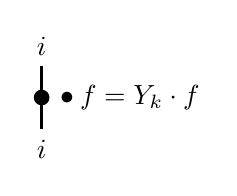
\begin{tikzpicture}[scale=.4,baseline]
\draw[very thick] (1,-1) -- (1,1) node[at start,below]{
$i$} node[at end,above]{
$i$} node[circle,midway,fill,inner sep=2pt]{};
\node at (3.8,0) {$\bullet\: f= Y_k\cdot f$ } ;
\end{tikzpicture}
  \end{equation*}
\begin{equation*}
  \begin{tikzpicture}[scale=.4]
\draw[very thick] (1,-1) -- (-1,1) node[at start,below]{
$j$} node[at end,above]{
$j$};
\draw[very thick] (-1,-1) -- (1,1) node[at start,below]{
$i$} node[at end,above]{
$i$};
\node at (7.5,0) {$\bullet\: f=\begin{cases}
 P_{ji}(Y_k,Y_{k+1}) f^{s_k} & i\neq j\\
 \displaystyle \frac{f^{s^k}- f}{Y_{k+1}-Y_{k}} & i=j  
\end{cases}$ } ;
\end{tikzpicture}
\end{equation*}
\end{lemma}}


Given a choice of $\phi$ corresponding to an element of $\fg_{\Bw}$, we let $\phi_{i,1},\dots, \phi_{i,w_i}$ be the eigenvalues of this element acting on $W_i$; for simplicity, we assume these are all integral.  We let $\ell$ be the number of distinct values of $\phi_{i,k}$ for all $i$ and $k$, and choose a numbering of these values. If $\phi_{i,k}$ is the $m$th such value,  we let $\theta_m=\frac{\phi_{i,k}+\nicefrac{1}{2}}{p}$. For simplicity, we assume that our quiver $\Gamma$ has no oriented cycles, so there is an order on vertices such that arrows always point in the increasing direction.  We call an object in the cylindrical KLR category $\boldsymbol{\theta}$-compatible if it can be isotoped to have $x$-values in the regions $[a/p,a/p+\delta]$ for $a\in \Z/p\Z$ and $\delta>0$ arbitrarily small, with the labels on strands in this region weakly increasing from left to right in each of these regions. 

Recall that for us, a choice of weight $\beta\in \ft_{1,\Fp}$ is choosing a $\beta_{i,k}\in \Fp$ for each $i\in \Gamma$ and $k\in [1,v_i]$; the corresponding element of $\ft_{1,\Fp}\subset \fg_{\Bv}\oplus \fg_{\Bw}$ has component in $\mathfrak{gl}(v_i)$ defined by $\operatorname{diag}(\beta_{i,1},\dots \beta_{i,v_i})$, and $\mathfrak{gl}(w_i)$ by $\operatorname{diag}(\phi_{i,1},\dots, \phi_{i,w_i})$.
Thus, note that $ \frac{\beta_{i,k}}{p}\in \R/\Z$ is well-defined. 
\begin{theorem}\label{thm:KLR-equiv}
The category $\pStein_\Fp$ is equivalent to the subcategory of
$\boldsymbol{\theta}$-compatible objects in the cylindrical KLR category, sending a weight $\beta$ to the object where a black strand with label $i$ is placed in the region $[\beta_{i,k},\beta_{i,k}+\delta]$ for each $i\in \Gamma, k\in [1,v_i]$, with the strands in each of these regions ordered in increasing order.
\end{theorem}
\begin{proof}
First we must describe the image of generators under this functor. \begin{itemize}
\item The weight $\varepsilon_{i,k}$ of action on the $k$th basis vector in $\C^{v_i}$ is sent to the action of the dot on the associated strand.
\item If $s_{i,k}\cdot \beta=\beta$, then we have $\beta_{i,k}=\beta_{i,k+1}$, so the corresponding strands are adjacent, and we send $\psi_{i,k}$ to the crossing of these strands with the same label.
\item The action of elements of the affine Weyl group only reorders the strands in one neighborhood of $[\beta_{i,k}/p,\beta_{i,k}/p+\delta]$ that have the same label; we do this using the ``neutral crossing'' $\al_{i,k}\psi_{i,k}+1$
\item Using the elements of the affine Weyl group, we have reduce to describing the image of $\wall(\beta,\beta')$ with the two endpoints in the same Weyl alcove.  In this case, we simply draw the straightline diagram such that the strand associated to $(i,k)$ changes $x$-value by $(\beta_i-\beta_i')/p$; this never crosses two strands with the same label, since we never change alcove.  The elements $\wall(\beta,\beta')$ that do change alcoves just have to use the ``neutral crossing'' $\al_{i,k}\psi_{i,k}+1$ when we change alcoves. 
\end{itemize} 
That this matches the representation (\ref{Y-action})  is a straight forward calculation in the usual mold.  It's worth noting that the weights of the representation that appear are either of the form $\varepsilon_{i,k}$ or $\varepsilon_{i,k}-\varepsilon_{j,m}$ if there is an edge $j\to i$.  The multiplication by the former in \ref{Y-action} is accounted for by red/black crossings and (\ref{cost}), and by the latter by black/black crossings and (\ref{black-bigon}).  This gives a functor from the $\boldsymbol{\theta}$-compatible objects to  $\pStein_\Fp$ which is easily seen to be full.  We this is an equivalence comparing the usual basis $w\tilde{r}(w^{-1}\eta',\eta)$ of morphisms in $\pStein_\Fp$ with that of Lemma \ref{lem:cyl-basis}.
\end{proof}
Implicitly, this tells us that we have an equivalence between the
representation category $\widehat{\BFN}$ for $\Fp$ and the
$\boldsymbol{\theta}$-compatible objects in the cylindrical KLR
category.  We send the sequence $\Bi$ and eigenvalues $\Ba$ to placing
elements with label $i_k$ at $a_k/p+k\delta/n$.  We map the diagrams
to the usual ones suggested by the polynomial representations.
%\begin{equation*}
%  y_k\mapsto y_k+a_k\qquad 
%\end{equation*}




In certain applications, it is more natural to consider a weighted
cylindrical KLR algebra.  This is sufficiently abstruse that we feel a
lengthy discussion would only confuse matters.  One can define {\bf
  weighted KLR diagrams} for a weighting on the quiver $\Gamma$, which
follow the local rules defined in \cite{WebwKLR}: for each edge $e$ of
weight $\vartheta_e$, and each strand with label $h(e)=i$ we add a
``ghost'' shifted $\vartheta_e$ units to the right (or left if
$\vartheta_e$ is negative).  We require that there are no tangencies or triple
intersection points between any combination of strands and ghosts, and
no dots on intersection points. 
We'll consider these diagrams up to isotopy which preserves all these
conditions.  The {\bf cylindrical weighted KLR algebra} is obtained by
quotienting the formal span of such diagrams by the local relations of
\cite[Def. 2.4]{WebwKLR} instead of (\ref{first-QH}--\ref{cost})
above. 

For a general $\phi$, we also have to include a weight along each
edge, which we denote $\vartheta_e$.  Note that when we choose $\ep_i$, invariance under the Weyl group
requires that we assign the same value to all the weights coming from
the matrix coefficients of the map along a given edge.  Thus, we can
just think of this as a value attached to each edge as well, which we
denote $\ep_i$.  
\begin{lemma}\label{lem:weighted-pStein}
The category $\pStein_\Fp'$ is equivalent to the weighted cylindrical
KLR category with the weight of each edge given by $\vartheta_e+\ep_e$.  The category $\pStein_\Fp$ is equivalent to the subcategory of $\boldsymbol{\theta}$-compatible objects for the weighted cylindrical category with weights $\ep_i$.  
\end{lemma}




\subsection{Reduction from the linear case}
\label{sec:reduct-from-line}
Recall that in \cite[\S 4]{Webmerged}, we defined an algebra $\tilde{T}^{\bla}$ which is defined by Stendhal diagrams in $\mathbb{R}\times [0,1]$ modulo the same local relations (\ref{first-QH}--\ref{cost}); as in the cylindrical case, we can think of this interchangably as a category, and we will use the same notation for the category and algebra.  Since these relations are independent of isotopy, we can assume that we have shrunk our diagrams to lie in $(0,1)\times [0,1]$, and placed the red lines at $x=\tilde{\theta}_i$, the unique lifts of $\theta_i$ to this interval, which are in increasing order.  Thus, considering their image under the natural map $ (0,1)\times [0,1]\to \R/\Z\times [0,1]$ induces a ring homomorphism $\tilde{T}^{\bla}\to \mathring{R}$.  
Lemma \ref{lem:cyl-basis} shows that $\mathring{R}$ is a free $\tilde{T}^{\bla}$-module, so pushforward by this homomorphism is an exact functor which sends projectives to projectives.  In fact, we can view $\mathring{R}$ as constructed directly from $\tilde{T}^{\bla}$.  If a category $\mathcal{B}$ has both a left and right action of an monoidal category $\mathcal{C}$, we can take the trace $\Tr_{\mathcal{C}}\mathcal{B}$ of this categorical bimodule by formally adjoining an isomorphism between the bifunctors that send $(B,C)$ to $B\otimes C$ and $C\otimes B$.  Note that the result is a category which has neither a left nor right $ \mathcal{C}$-module structure.

The KLR algebra acts on the category $\tilde{T}^{\bla}$ by adding black terminals at the left and the right, as discussed in \cite[\S 2.2.3]{Webweb}.
\begin{proposition}
The cylindrical KLR category $\mathring{R}$ is the trace $\Tr_{R}\tilde{T}^{\bla}$ of $\tilde{T}^{\bla}$ for the left and right actions of the standard linear KLR category $R$.  Similarly, the derived category $D^b(\mathring{R})$ is the trace of the corresponding bimodule structure for the derived category of $\tilde{T}^{\bla}$ over that of $R$. 
\end{proposition}
 The new isomorphism between the left and right actions of an object is the cylindrical Stendhal diagram which sends those strands around the back of the cylinder (i.e. passing through the seam in our usual way of drawing diagrams).  


We can also construct the BFN/KLR algebra in a similar method, but after some appropriate modifications.  Consider the deformed weighted KLR category $\tilde{\mathbb{T}}^{\la_1}$ defined by Stendhal diagrams with a single red strand at $x=\epsilon$ for $0<\epsilon\ll 1$, modulo the KLR relations (\ref{b-first-QH}--\ref{b-triple-smart}) and the deformed red/black relations:
\newseq
    \begin{equation*}\subeqn\label{T-dot-slide}
    \begin{tikzpicture}[very thick,baseline,scale=.7]
  \draw(-3,0) +(-1,-1) -- +(1,1);
  \draw[wei](-3,0) +(0,-1) -- +(0,1);
\fill (-3.5,-.5) circle (3pt); \end{tikzpicture}
=
 \begin{tikzpicture}[very thick,baseline,scale=.7] \draw(1,0) +(-1,-1) -- +(1,1);
  \draw[wei](1,0) +(0,-1) -- +(0,1);
\fill (1.5,.5) circle (3pt);
    \end{tikzpicture}
\qquad \qquad     \begin{tikzpicture}[very thick,baseline,scale=.7]
  \draw(-3,0) +(1,-1) -- +(-1,1);
  \draw[wei](-3,0) +(0,-1) -- +(0,1);
\fill (-2.5,-.5) circle (3pt); \end{tikzpicture}
=
 \begin{tikzpicture}[very thick,baseline,scale=.7] \draw(1,0) +(1,-1) -- +(-1,1);
  \draw[wei](1,0) +(0,-1) -- +(0,1);
\fill (.5,.5) circle (3pt);
    \end{tikzpicture} 
  \end{equation*}
 \begin{equation*}\subeqn\label{T-cost}
  \begin{tikzpicture}[very thick,baseline,scale=.7]
    \draw (-2.8,0)  +(0,-1) .. controls (-1.2,0) ..  +(0,1) node[below,at start]{$i$};
       \draw[wei] (-2,0)  +(0,-1)--  +(0,1);
  \end{tikzpicture}
=   p_{i,-}\Bigg(
  \begin{tikzpicture}[very thick,baseline,scale=.7]
 \draw[wei] (2.3,0)  +(0,-1) -- +(0,1);
       \draw (1.5,0)  +(0,-1) -- +(0,1) node[below,at start]{$i$};
       \fill (1.5,0) circle (3pt);
\end{tikzpicture}\hspace{5mm}\Bigg)\qquad \qquad
  \begin{tikzpicture}[very thick,baseline,scale=.7]
          \draw[wei] (-2,0)  +(0,-1)-- +(0,1);
  \draw (-1.2,0)  +(0,-1) .. controls (-2.8,0) ..  +(0,1) node[below,at start]{$i$};\end{tikzpicture}
           =p_{i,-}\Bigg(\hspace{5mm}
  \begin{tikzpicture}[very thick,baseline,scale=.7]
    \draw (2.5,0)  +(0,-1) -- +(0,1) node[below,at start]{$i$};
       \draw[wei] (1.7,0)  +(0,-1) -- +(0,1) ;
       \fill (2.5,0) circle (3pt);\end{tikzpicture}\Bigg)
\end{equation*}
\begin{equation*}\subeqn\label{T-triple-smart}
    \begin{tikzpicture}[very thick,scale=.9,baseline]
      \draw (-3,0) +(1,-1) .. controls (-4,0) .. +(-1,1) node[below,at start]{$i$}; \draw
      (-3,0) +(-1,-1) .. controls (-4,0) .. +(1,1) node[below,at start]{$i$}; \draw[wei]
      (-3,0) +(0,-1)--  +(0,1); \node at (-1,0) {=}; \draw (1,0) +(1,-1) .. controls
      (2,0) .. +(-1,1)
      node[below,at start]{$i$}; \draw (1,0) +(-1,-1) .. controls
      (2,0) .. +(1,1)
      node[below,at start]{$i$}; \draw[wei] (1,0) +(0,-1) -- +(0,1); \node at (2.8,0)
      {$+$};        \draw (6.2,0)
      +(1,-1) -- +(1,1) node[below,at start]{$i$}; \draw (6.2,0)
      +(-1,-1) -- +(-1,1) node[below,at start]{$i$}; \draw[wei] (6.2,0)
      +(0,-1) -- +(0,1); 
\node[inner ysep=8pt,inner xsep=5pt,fill=white,draw,scale=.8] at (6.2,0){$\displaystyle \frac{p_{i,-}(y_1)-p_{i,-}(y_2)}{y_1-y_2}$};
    \end{tikzpicture}
  \end{equation*}
\begin{equation*}\subeqn\label{T-triple-dumb}
    \begin{tikzpicture}[very thick,scale=.9,baseline]
      \draw (-3,0) +(1,-1) .. controls (-4,0) .. +(-1,1) node[below,at start]{$j$}; \draw
      (-3,0) +(-1,-1) .. controls (-4,0) .. +(1,1) node[below,at start]{$i$}; \draw[wei]
      (-3,0) +(0,-1)--  +(0,1); \node at (-1,0) {=}; \draw (1,0) +(1,-1) .. controls
      (2,0) .. +(-1,1)
      node[below,at start]{$j$}; \draw (1,0) +(-1,-1) .. controls
      (2,0) .. +(1,1)
      node[below,at start]{$i$}; \draw[wei] (1,0) +(0,-1) -- +(0,1); 
    \end{tikzpicture}
\qquad \text{if $i\neq j$.}
  \end{equation*}
This also has left and right actions of the KLR category for the polynomials $q_{ij}$. Let $\Sigma$ be the autofunctor of the KLR category  that preserves
every object and dotless diagram, and sends every dot to that dot plus $h$.
Note that this is only well defined because $q_{ij}(u\pm h,v\pm h)=q_{ij}(u,v).$


\begin{definition}
The {\bf twisted trace} of a category $\mathcal{B}$ with both a left and right action of an monoidal category $\mathcal{C}$, with respect to a weakly monoidal autofunctor $\Sigma$ by formally adjoining an isomorphism between the bifunctors that send $(B,C)$ to $B\otimes C$ and $\Sigma(C)\otimes B$.  
\end{definition} 

\begin{proposition}
The cylindrical BFN category attached to these polynomials is equivalent to the twisted trace of $\tilde{\mathbb{T}}^{\la_1}$ with respect to the functor $\Sigma$.
\end{proposition}
\begin{proof}
Every object in the twisted trace is isomorphic one with a red strand
at the far left.  We turn this into a slice in cylinder by matching
the red strand to $x=\epsilon$ and placing
black strands accordingly in the interval $(\epsilon,1)$.  
Morphisms between these objects are generated by ones of a simple form:
\begin{enumerate}
    \item Diagrams
in $\tilde{\mathbb{T}}^{\la}$ that never crosses the red
strand.  These we simply compress using an isotopy into $(\epsilon,1)$ and hen map into the cylinder.
\item The diagram which wraps a single strand past the  red strand,
and then uses the trace relation to move it to the right or vice versa. This we send to the cylindrical diagram simply crossing $x=0$.
\end{enumerate}
Now, we need to check that this matches the relations.  The KLR relations (\ref{b-first-QH}--\ref{b-triple-smart}) are the same thus obviously match.  
 The relations
(\ref{dot-slide}--\ref{x-triple-dumb}) and (\ref{T-dot-slide}--\ref{T-triple-dumb}) don't match directly, but they do if one applies $\Sigma^{-1}$ to the dots on the left side of the red line in (\ref{T-dot-slide}--\ref{T-triple-dumb}).
\end{proof}


If both $\mathcal{B}$ and $\mathcal{B}'$ have bi-actions of $ \mathcal{C}$, then we say that a functor $F\colon \mathcal{B}\to \mathcal{B}'$ commutes with these actions if we have isomorphisms $F(C\otimes B\otimes C')\cong C\otimes F(B)\otimes C'$ natural in $B, C$, and $C'$.
The construction of (twisted) trace is obviously natural for functors commuting with the $\mathcal{C}$ bi-action: the isomorphism $B\otimes C\cong C\otimes B$ is sent to the same for $F(B)\otimes C$ and $C\otimes F(B)$.

There are a couple of interesting such functors.  The first is the braid group action defined in \cite[\S 5]{Webmerged}.  These are defined by tensor product with bimodules $\mathfrak{\tilde B}_\sigma$. That these commute with the left and right action is proven as in \cite[Prop. 6.7]{Webmerged}; that result covers the bimodule $\mathfrak{ B}_\sigma$ with the violating relation added, but the proof is unchanged.  Let us describe the cylindrical analogues of these bimodules.  Let $\vartheta,\vartheta'\in \R^\ell$ be real lifts of the positions of the red strands.  
Fix an extended affine permutation $w\in \widehat{S}_n$. 
\begin{definition}
 Let $\mathring{\mathfrak{B}}_w$ be the bimodule spanned by modified Stendhal diagrams where the red lines trace out a reduced string diagram for $w$, and the black strands still follow the rules of Definition \ref{def:cyl-Stendhal}, modulo the local relations (\ref{first-QH}--\ref{cost}) and the local relations 
 \newseq
 \begin{equation*}\label{side-dumb}\subeqn
    \begin{tikzpicture}
      [very thick,scale=1,baseline] \usetikzlibrary{decorations.pathreplacing}
      \draw[wei] (1,-1) -- (-1,1) node[at start,below]{$\la_k$}
      node[at end,above]{$\la_k$} node[midway,fill=white,circle]{};
      \draw[wei] (-1,-1) -- (1,1) node[at start,below]{$\la_{k+1}$}
      node[at end,above]{$\la_{k+1}$}; \draw (0,-1)
      to[out=135,in=-135] (0,1); \node at (3,0){=}; \draw[wei] (7,-1)
      -- (5,1) node[at start,below]{$\la_k$} node[at
      end,above]{$\la_k$} node[midway,fill=white,circle]{}; \draw[wei] (5,-1)
      -- (7,1) node[at start,below]{$\la_{k+1}$} node[at
      end,above]{$\la_{k+1}$}; \draw (6,-1) to[out=45,in=-45] (6,1);
    \end{tikzpicture}.
  \end{equation*}
  \begin{equation*}\label{top-dumb}\subeqn
    \begin{tikzpicture}
      [very thick,scale=1,baseline] \usetikzlibrary{decorations.pathreplacing}
      \draw[wei] (1,-1) -- (-1,1) node[at start,below]{$\la_k$}
      node[at end,above]{$\la_k$} node[midway,fill=white,circle]{};
      \draw[wei] (-1,-1) -- (1,1) node[at start,below]{$\la_{k+1}$}
      node[at end,above]{$\la_{k+1}$}; \draw (1.8,-1)
      to[out=145,in=-20] (-1,-.2) to[out=160,in=-80] (-1.8,1); \node
      at (3,0){=}; \draw[wei] (7,-1) -- (5,1) node[at
      start,below]{$\la_k$} node[at end,above]{$\la_k$}
      node[midway,fill=white,circle]{}; \draw[wei] (5,-1) -- (7,1) node[at
      start,below]{$\la_{k+1}$} node[at end,above]{$\la_{k+1}$}; \draw
      (7.8,-1) to[out=100,in=-20] (7,.2) to[out=160,in=-35] (4.2,1);
    \end{tikzpicture}.
  \end{equation*}
  \begin{equation*}\label{triple-point-red}\subeqn
    \begin{tikzpicture}
      [very thick,scale=1,baseline] \usetikzlibrary{decorations.pathreplacing}
      \draw[wei] (1,-1) -- (-1,1) node[at start,below]{$\la_{k-1}$}
      node[at end,above]{$\la_{k-1}$};
 \draw[white,line width=7pt] (0,-1) .. controls (1,0) .. (0,1);
 \draw[wei] (0,-1) .. controls (1,0) .. (0,1) node[at start,below]{$\la_{k}$}
      node[at end,above]{$\la_{k}$};
  \draw[white,line width=7pt] (-1,-1) -- (1,1);
      \draw[wei] (-1,-1) -- (1,1) node[at start,below]{$\la_{k+1}$}
      node[at end,above]{$\la_{k+1}$}; 
\node
      at (3,0){=};       \draw[wei] (7,-1) -- (5,1) node[at start,below]{$\la_{k-1}$}
      node[at end,above]{$\la_{k-1}$};
 \draw[white,line width=7pt] (6,-1) .. controls (5,0) .. (6,1);
 \draw[wei] (6,-1) .. controls (5,0) .. (6,1) node[at start,below]{$\la_{k}$}
      node[at end,above]{$\la_{k}$};
  \draw[white,line width=7pt] (5,-1) -- (7,1);
      \draw[wei] (5,-1) -- (7,1) node[at start,below]{$\la_{k+1}$}
      node[at end,above]{$\la_{k+1}$}; 
    \end{tikzpicture}.
  \end{equation*}
  We let $\mathring{\mathbb{B}}_w$ be the functor of derived tensor product with this module.  
\end{definition}
Note that the cylindrical KLR algebras acting at the top and bottom correspond to the sequences of weights $\bla$ and $w\cdot \bla$ respectively.  

\begin{lemma}\label{lem:w-basis}
  The bimodule $\mathring{\mathfrak{B}}_w$ has a basis over the action of dots on the left given by dotless diagrams tracing out the different affine permutations, drawn with a minimal number of crossings.
\end{lemma}

\begin{proposition}\label{prop:ring-reduce}
If $w\in S_n$, then the functor $\mathring{\mathbb{B}}_w$ coincides with that induced by the functor $\tilde{\mathbb{B}}_w$ for the linear algebra $\tilde{T}^\bla$.
\end{proposition}
\begin{proof}
It suffices to compare these functors on the algebra $\mathring{R}^\bla$ itself.  That is, we have to establish an isomorphism between $\mathring{\mathfrak{B}}_w$ and the image of $\tilde {\mathfrak{B}}_w$ under reduction.  We can map this reduction to $\mathring{\mathfrak{B}}_w$ as discussed earlier by sending the left-to-right isomorphism as the diagram passing around the back of the cylinder. Draw the basis from \ref{lem:w-basis} using  isotopies to move all strands passing around the back to the top of the diagram above all the red-red crossings. These vectors are obviously in the image of the map, which shows that it is surjective.  On the other hand, every diagram in the reduction of $\tilde {\mathfrak{B}}_w$ can be written in this form just using the relations of $\tilde{T}^\bla$; the fact that these vectors remain independent in $\mathring{\mathfrak{B}}_w$ shows that the map must be injective as well.
\end{proof}

Let $\rho\in \hat{W}_n$ be the length 0 affine permutation sending every integer $i$ to $i+1$;  this rotates each red line one click to the right.  Note that $\rho^m s_i=s_{i+m}\rho^m$.  
\begin{theorem}\label{thm:B-braid-action}
 The functors $\mathbb{\mathring{B}}_{s}$ for $s$ of length 0 or 1 define an action of the extended affine braid group of $S_n$ on the categories $\sum_{w\in S_n}D^b(\mathring{R}^{w\cdot \bla}\mmod)$.
\end{theorem}
Obviously, one can grade this module for the KLR and odometer gradings (with red-red crossings having degree 0 in both).  
\begin{proof}
Length 0 elements just correspond to cyclic permutations of the labels on red strands, so up to isotopy they are trivial and thus the relation $\mathbb{B}_{\rho^m}  \mathbb{B}_{s_i}=\mathbb{B}_{s_{i+m}} \mathbb{B}_{\rho^m}$ is clear.   It only remains to show that the braid relations hold for length 1 elements.  For any given braid relation, we can write all the functors involved as reductions from a single $\tilde{T}^{\bla}$ (since there is at least one vertical line that they do not have any crossings over).  Thus, we are just using the fact that  reducing functors is compatible with composition.
\end{proof}


More generally
\excise{Thus we have an induced isomorphisms:
\begin{equation}\label{lem:Frob-split}
  \Hom_{\mathsf{B}}(\second,\second)\cong \K[\hat{\fM}]
\end{equation}
\begin{proof}

\end{proof}


In fact, we can construct $e_\mu\hat{\Isalg}_\phi e_{\mu'}$ as the reduction of an appropriate sum of Hom spaces in the corresponding category for the Coulomb branch of $\To$. An important special case of this is  the module $\hat{Q}_{\tilde{\mu}}=\Hom_{\widehat{\pStein}_{\To,\K}}(e_0\cdot \second, \tilde{\mu})$ for the larger quantum Coulomb branch $\EuScript{A}_H^{\operatorname{sph}}$.
This is independent of the choice of lift, since cocharacters that differ by an integral amount give isomorphic objects in $\EuScript{B}$.
The vector bundle $\mathcal{\hat Q}_\mu=e_{\mu}\hat{\Isalg}_\phi e_{\second,0}$ is the coherent sheaf on $\tilde{\fM}$ obtained by applying Hamiltonian reduction to this module to obtain a coherent sheaf on $\tilde{\fM}$. }

We can consider the same Hamiltonian reduction applied before completion.  The result is a coherent sheaf ${\mathcal{Q}}_\mu$ which is equivariant for $\bS$ and whose restriction to $\hat{\fM}$ is isomorphic to $\hat{\mathcal{Q}}_\mu$.  Semi-continuity implies that ${\mathcal{Q}}_\mu$ is locally free of rank $\#W$.

\begin{lemma}\label{lem:pStein-fully-faithful}
  There is a fully faithful functor $\pStein_\K\to \Coh(\tfM)$ sending $\mu\mapsto {\mathcal{Q}}_\mu$.  
\end{lemma}
\begin{proof}
  The existence of a functor follows from the fact that the spaces ${Q}_{\tilde{\mu}}$ are a representation of the category ${\pStein}_{H,\K}$, so their reduction is one of the reduced category ${\pStein}_{\K}$.  
  
  By Lemma \ref{lem:Gamma-iso}, this functor is fully faithful after completion.  In particular, since $\pStein_\K$ injects into its completion, the functor is faithful.
  
  The grading on ${\pStein}_{\K}$ is compatible with a $\bS$-equivariant structure on ${Q}_{\tilde{\mu}}$, so the cokernel of the map on morphisms is also $\bS$-equivariant, and since the map is full after completion, its restriction to $\hat{\fM}$ is trivial.  Thus, by semi-continuity, this cokernel is trivial, and the functor is full. 
\end{proof}

In general, we can use Theorem \ref{thm:pStein-equiv} to describe a bimodule over the categories $\pStein_\K$ for the different values of $\phi$, by writing both as ``Hamiltonian reductions'' of the category $\pStein_H$ associated the Coulomb branch for $\To$.  Let $\pSteinK$ be the quotient of $\pStein_H$ by the morphisms $\gk\subset \Sym(\gk)\subset  \Sym(\ft^*+\ft_H^*)$.  

The category $\pStein_\K$ for a fixed parameter $\phi$ can be obtained as a subcategory of $\pSteinK$ where we only consider objects 
lying in the coset of $\phi$. Considering the Hom spaces in $\pSteinK$ between objects in the coset of $\phi$ and that of $\phi'$ gives a bimodule ${}_{\phi'}\tau_{\phi}$ between these categories.  
Applying Theorem \ref{thm:pStein-equiv} in the case of $\EuScript{A}_{H}$ shows that:


\begin{theorem}
  The equivalence of Theorem \ref{thm:pStein-equiv} matches the bimodules ${}_{\phi'}T_{\phi}$ and ${}_{\phi'}\tau_{\phi}$.
\end{theorem}
We can also add in the action of the Weyl group using the induced equivalences between $\pStein_\K$ for $\phi$ and $w\phi$ for $w\in W_H$.

We will leave to another time an exploration of the general case of this result, but in the special case of a quiver variety, we will continue our program of reformulating these structures in terms of cylindrical KLR algebras.  For simplicity, we assume that we are using tensor product flavors, i.e. a choices of $\phi$ corresponding to elements $\mathfrak{g}_{\Bw}$.  

\begin{proposition}\label{prop:braidings-match}
  The isomorphism of Theorem \ref{thm:KLR-equiv} intertwines the
  bimodule ${}_{w\phi}T_{\phi}$ with the braiding bimodule $\mathfrak{B}_w$ associated to
  the positive braid lifting $w$.  
\end{proposition}
\begin{proof}
This follows immediately from applying the analogue of Theorem
\ref{thm:KLR-equiv} (which is an application of
\cite[Thm. 4.2]{WebSD}) for the Coulomb branch of $G_\Bw\times
G_{\Bv}$ acting on $E_{\Bv}^{\Bw}$.   
\end{proof}
Similarly, we can extend this to more general flavors in quiver gauge theories by using change-of-charge bimodules \cite[\S 2.5]{WebwKLR} and \cite[\S 5.3]{WebRou}.
